\documentclass[sommairechap,stylejchiquet]{these_gi}



\begin{document}

% ==================================================================
% OPTIONS D'AFFICHAGE
% non-d�finitif (soumis aux rapporteurs) ou  d�finitif
\definitiftrue
% \definitiffalse
 
% ==================================================================
% RENSEIGNEMENTS SUR LA TH�SE
\titleFR{D�codage des intentions et des repr�sentations motrices chez l'homme: analyse multi-�chelle et application aux interfaces cerveau-machine}
\titleEN{Le titre en anglais}
\abstractFR{Le r�sum� en fran�ais ($\approx$ 1000 caract�res)}
\abstractEN{Le r�sum� en anglais ($\approx$ 1000 caract�res)}
\keywordsFR{Les mots-cl�s en fran�ais}
\keywordsEN{Les mots-cl�s en anglais}
 
\author{Etienne Combrisson}
\address{e.combrisson@gmail.com}
\universite{universit� claude bernard lyon 1}
\laboratoire{}
\specialite{sp�cialit� de la th�se}
\datesoutenance{09/2016}
\datesoumission{la date de soumission aux rapporteurs}
\jury{\begin{tabular}{llll}
    M\up{me} & \textsc{Erika Rat�} & Universit� � la Menthe & (Rapporteur) \\
    M. & \textsc{Jacques Ouille} & Universit� � la Fraise & (Rapporteur) \\
    M. & \textsc{Henri Zoto} & Laboratoire laborieux & (Rapporteur) \\
    M. & \textsc{Jean File} & Indienne & (Directeur) \\
       & etc. &  \\
  \end{tabular}    
}
 
% ==================================================================
% D�DICACE
\dedicate{� Isabelle et Didier, mes deux parents,\\ qui ont tout donn� pour que ceci me soit un jour possible. \\ Merci}
 
% ==================================================================
% DEBUT DE LA PR�FACE
\beforepreface
 
% remerciements
\chapter*{Remerciements}

%% Encadrant
\malettrine{J}{e}  voudrais tout  d'abord exprimer  mes  plus profonds
remerciements �\dots AH���H !

% �lo�se
Je conclurai en  remerciant de tout c{\oe}ur (l'�tre aim�).

\vspace{2cm}

\hfill Montr�al, le \today.


 
% table des mati�res g�n�rale
\tableofcontents
 
% affiche la liste des figures
\newpage
\listoffigures

% ==================================================================
\afterpreface

% ==================================================================
% NOTATIONS
\chapter*{Notations}
\addcontentsline{toc}{chapter}{Notations}

\pagestyle{plain}

%----------------------------------
% GENERAL
%----------------------------------
\Large G\'en\'eral \\% \bigskip
\normalsize
\begin{supertabular}{ll}
  ICM & Interface Cerveau-Machine \\
  BCI & Brain Computer Interface \\
\end{supertabular}

%----------------------------------
% ENREGISTREMENTS
%----------------------------------
\vspace{1cm}
\Large Enregistrements \\% \bigskip
\normalsize
\begin{supertabular}{ll}
  EEG & \eeg \\
  MEG & \meg \\
  SUA & \sua \\
  MUA & \mua \\
  SEEG & \seeg \\
  ECoG & \ecog \\
\end{supertabular}

%----------------------------------
% FEATURES
%----------------------------------
\vspace{1cm}
\Large Features \\% \bigskip
\normalsize
\begin{supertabular}{ll}
  PAC & Phase Amplitude Coupling \\
\end{supertabular}

%----------------------------------
% CLASSIFIEURS
%----------------------------------
\vspace{1cm}
\Large Classifieurs \\% \bigskip
\normalsize
\begin{supertabular}{ll}
  LDA & \lda \\
  SVM & \svm \\
  RF & \rf \\
  KNN & \knn \\
  NB & \nb \\
\end{supertabular}

\chapterend

% ==================================================================
% AVANT-PROPOS
% *****************************************************************************
% *****************************************************************************
%                                   INTRODUCTION
% *****************************************************************************
% *****************************************************************************
\part{Introduction g�n�rale}
\pagestyle{headings}

\malettrine{B}{lablablabkiblablou}  INTRO \dots\\*

% Le sujet de la th�se
L'objectif de cette th�se a  �t� de \dots\\*

Totalit� des m�thodes explor�es durant ma th�se sont pr�sentes dans une toolbox python appel�e brainpipe, libre d'acc�s et de droit. 


% #############################################################################
%                                CORPS DE L'INTRO
% #############################################################################
% #############################################################################
%                        PRESENTATION DE LA THEMATIQUE
% #############################################################################
\chapter{Pr�sentation de la th�matique}

En 1964, Dr. Grey Walter connecte des �lectrodes directement dans le cortex moteur d'un patient et lui demande de presser un bouton pour faire avancer un r�tro-projecteur. En m�me temps, il enregistre l'activit� neuronale de telle sorte que elle aussi, puisse le faire avancer. L� o� l'exp�rience devient remarquable, c'est que le r�tro-projecteur avance avant que le patient ne presse le bouton ! Tout l'appareil musculaire du sujet est court-circuit� et le contr�le se fait sans mouvement. Contr�ler par la \textit{pens�e}, un sujet de science fiction qui devient une r�alit�.\\
Cette anecdote d�crite par \cite{graimann_braincomputer_2009}, permet de placer la naissance des \icm (ICM) dans l'histoire. C'est le point d'entr�e qui a ensuite conduit une grande diversit� de chercheurs � se passionner pour ce sujet. \\

% -----------------------------------------------------------------------------
% -> D�finition d'une ICM
\section{\icm: d�finition et objectifs}

\subsection{Interactions naturelles avec l'environnement}
Pour interagir avec son environnement, l'individu se sert des voies de communications naturelles, \cad via son syst�me nerveux et musculaire. Le processus de communication d�bute par une intention qui active certaines r�gions dans le cerveau. Il en r�sulte un signal c�r�brale qui est ensuite envoy� par le syst�me nerveux p�riph�rique en directions des muscles. C'est ce processus simplifi� qui permet � une personne d'interagir avec ce qui l'entoure.

\subsection{ICM: une communication alternative}
Une ICM (ou BCI en anglais pour \textit{Brain Computer Interface}) est un autre syst�me de communication o� les voies naturelles sont cout-circuit�es. Au lieu de passer par le syst�me nerveux puis musculaire, le signal c�r�bral est directement intercept� au niveau du cerveau et va ensuite �tre transform� en commandes. Une ICM est donc un syst�me permettant de traduire une activit� neuronale en commande ext�rieure. Le terme \textit{traduire} est � prendre au sens linguistique \cad que les signaux c�r�braux forment un langage, compos� de r�gles, de motifs ou \textit{pattern}, que l'on va essay� de d�coder (via un ordinateur) pour les transformer en op�rations. D'o� le terme "\icm".

\subsection{Composantes d'une ICM}
\cite{pfurtscheller_rehabilitation_2008} et \citep{graimann_braincomputer_2009} introduisent quatre �l�ments qui composent une ICM:
\begin{enumerate}
	\item Enregistrer l'activit� directement depuis le cerveau. Cet enregistrement pourra �tre invasif ou non-invasif (cf. \ref{invasif_non-invasif})
	\item G�n�rer un retour ou \textit{feedback} pour l'utilisateur
	\item L'enregistrement et le \textit{feedback} doivent �tre en temps r�el
	\item Enfin, l'interface doit �tre contr�lable par l'utilisateur, de mani�re active, via un ensemble d'intentions. 
\end{enumerate}
A titre d'exemple et pour illustrer ce dernier point, un utilisateur pourrait par exemple d�cider de bouger un curseur de souris sur un �cran en imaginant des mouvements soit de la main gauche soit de la main droite.

\figScaleDesciption{0.7}{Pfurtscheller2008_SchemaICM}{Sch�ma d'une \icm \citep{pfurtscheller_rehabilitation_2008}}{L'activit� neuronale est enregistr�e (Signal acquisition) puis nettoy�e (Preprocessing). Ensuite, on extrait des motifs ou patterns qui caract�risent la commande que souhaite envoyer le sujet (Feature extraction). Enfin, la machine tente de reconna�tre ces motifs (Classification) et de les transformer en commande (Application interface) \citep{pfurtscheller_rehabilitation_2008}}

\subsection{Acquisition de l'activit� neuronale}
L'acquisition de l'activit� neuronale constitue la premi�re �tape d'une ICM. Deux param�tres permettent de d�crire ces diff�rentes techniques:
\begin{enumerate}
	\item L'accessibilit�: \cad si cette technique est plus ou moins facile � mettre en place. 
	\item La qualit�: \cad le rapport signal sur bruit (RSB)
\end{enumerate}
Si la technique d'enregistrement n'est pas facilement accessible, cela pourrait limiter le nombre de sujets potentiel pour l'�tude. La qualit� quant � elle va permettre d'avoir acc�s � des signaux c�r�braux de plus ou moins grande qualit� ce qui va influer sur la performance et sur les limitations d'une ICM. \\
Les diff�rents types d'acquisition peuvent �tre diff�renci�s par leur degr�s de p�n�tration dans le corps. Les enregistrements dits \textit{invasifs} vont n�cessiter une intervention chirurgicale mais donnent acc�s � des signaux de grande qualit�. Les enregistrements \textit{non-invasifs} sont globalement plus faciles � mettre en place car ne n�cessitant aucune chirurgie mais la qualit� du signal est moindre car l'activit� neuronale est enregistr�e en dehors de la bo�te cr�nienne. \\
Au sein de ces deux cat�gories, on trouvera un ensemble de m�thodes d'acquisition qui se diff�rencient par la taille des populations de neurones qu'elles enregistrent ou par le type de signal.

\subsubsection{Enregistrements invasifs}
On parlera d'intracr�nien pour les enregistrements � l'int�rieur de la bo�te cr�nienne puis d'intracortical pour des �lectrodes implant�es dans le cortex \citep{jerbi_task-related_2009, engel_invasive_2005}. �tant donn� que les techniques ci-dessous n�cessitent une intervention chirurgicale, \\

\textbf{\sua (SUA)} et \textbf{\mua (MUA)} : ces micro-�lectrodes d�pos�es directement au contact de neurones, disposent de la plus haute r�solution et enregistrent des d�charges neuronales. SUA et MUA se distinguent par la taille des populations enregistr�es.\\

\textbf{\seeg (SEEG)} : macro-�lectrodes enregistrant des populations plus larges que les micro-�lectrodes. contrairement � la SUA ou MUA o� l'on peut compter le nombre de fois qu'un ou plusieurs neurones d�chargent, la SEEG enregistre des potentiels �lectriques $(\mu V)$. \\

\textbf{\ecog (ECoG)} : grille flexible compos�e d'une matrice d'�lectrodes. Cette grille est ensuite d�pos�e � la surface corticale. Parce que cette m�thode n'est pas intracortical elle est dite \textit{semi-invasive}.

\subsubsection{Enregistrements non-invasifs}
Les m�thodes \textit{non-invasives} repr�sentent le but ultime de l'impl�mentation concr�te d'une \icm. En effet, ne n�cessitant aucune intervention chirurgicale, leur utilisation est tr�s r�pandue. Actuellement, bien qu'ayant une bonne r�solution temporelle permettant ainsi de capturer les ph�nom�nes courts, elles souffrent encore d'un manque de r�solution spatiale et d'un rapport signal sur bruit plus faible que les techniques invasives. \\

\textbf{\eeg (EEG)} : c'est la technique la plus utilis�e dans le domaine des ICM pour son aspect pratique et portatif. On dispose � la surface de la bo�te cr�nienne un ensemble d'�lectrodes qui enregistrent l'activit� �lectrique �manant de populations larges de neurones. On trouve m�me denouveaux syst�mes sans fils, prometteurs.\\

\textbf{\meg (MEG)} : autre m�thode \textit{non-invasive} mais nettement moins portable que l'EEG, la MEG enregistre les champs magn�tiques r�sultant de l'activit� �lectrique du cerveau. Ces champs magn�tiques peuvent �tre jusqu'� 10 milliards de fois plus faibles que le champs magn�tique terrestre. L'aspect inamovible de la MEG limite son utilisation pour les ICM mais on trouve quand m�me quelque �tudes ayant test� son utilisation \citep{mellinger_meg-based_2007, waldert_hand_2008}.

\figScaleDesciption{1}{Waldert_2009_recording}{M�thodes d'acquisition de l'activit� c�r�brale \citep{waldert_review_2009}}{M�thodes d'acquisition de l'activit� c�r�brale \citep{waldert_review_2009} class�es par invasivit�. La figure indique �galement la taille des populations de neurones enregistr�s ainsi que la r�solution spatiale intimement li�e � l'invasivit�.}

\subsection{Neuro-r�habilitation et handicap moteur}
Pr�lever directement l'activit� neuronale et donc, \textit{bypasser} les voies naturelles, permet de s'affranchir d'�ventuelles limitations physiologiques. C'est pourquoi les ICM repr�sentent un enjeu majeur pour la r�habilitation motrice ou handicap moteur ou encore pour la communication palliative.
Les applications concr�tes des \icm visent donc les personnes disposant de leurs capacit�s cognitives mais qui sont priv�es de facult�s motrices. \\
Par exemple, le \textit{syndrome d'enfermement} ou \textit{locked-in syndrome} qui surviennent majoritairement � la suite d'un accident vasculaire c�r�brale. Les personnes touch�es par ce syndrome sont pleinement consciente de leur corps, de l'environnement, ils peuvent ressentir les sensations de toucher et de douleur mais n'ont plus de facult�s motrices, hormis peut-�tre, les mouvements de paupi�res ou des yeux. Un autre exemple est celui de la la scl�rose lat�rale amyotrophique (ou SLA) qui est une d�g�n�rescence des neurones moteur. Progressivement, les personnes atteintes de SLA perdent l'usage des bras, des jambes, de la parole des muscles faciaux et enfin de la d�glutition. Toutefois, a l'instar du \textit{locked-in syndrome}, la conscience et les facult�s cognitives demeurent intactes. \\

SLA et \textit{locked-in syndrome} ne sont que deux exemples expliquant l'int�r�t social du d�veloppement des ICM. Redonner un peu de contr�le ou �tablir un canal de communication avec les familles des patients expliquent l'engouement qui existe depuis maintenant plus de 40 ans pour les ICM.

% Une description d�taill�e des ICM existantes est propos�e dans la section \ref{etat_de_lart_ICM}.


% -----------------------------------------------------------------------------
% Etat de l'art
\section{�tat de l'art des interfaces cerveau-machine}
\label{etat_de_lart_ICM}

Mettre des ICM plus r�centes voir faire un sch�ma r�capitulatif � mettre en annexe. Good idea

\citep{bekaert_les_2009}
\figScale{bekaert_2009_ICM}{Pipeline g�n�ral d'un \icm}

\subsection{Les diff�rents types d'\icm}
Okokok, ref vers ces diff�rents types
\subsubsection{ICM \textit{synchrones} et \textit{asynchrones}}
Intro blabla \\
\textbf{ICM \textit{synchrones}: } description\\
\textbf{ICM \textit{asynchrones}: } description

\subsubsection{ICM \textit{invasives} et \textit{non-invasives}}
\label{invasif_non-invasif}
Blabla intro \\
\textbf{ICM \textit{invasives} :} description \\
\textbf{ICM \textit{non-invasives} :} description \\
La partie qui va suivre introduit les diff�rents types d'enregistrement c�r�braux.

\subsection{ICM non-invasives}
P300 speller

\subsection{ICM invasives}
\citep{hochberg_reach_2012}
\figScale{hochberg_2012}{Contr�le d'un bras robotis�}

% -----------------------------------------------------------------------------
\section{Apprentissage machine: applications aux neurosciences}
okok

% -----------------------------------------------------------------------------
\section{Encodage et d�codage moteur: bases physiologiques}
Pomper les r�sultas de rodrigo + besserve + inclure sch�ma global du cerveau

% -----------------------------------------------------------------------------
\section{Intention, ex�cution et imagerie motrice}
La figure \ref{fig:hanakawa_2008}   repr�sente  une   trajectoire  d'un
processus markovien de saut, avec les notations associ�es.
\citep{hanakawa_motor_2008}
\figScale{hanakawa_2008}{Comparatif}

% -----------------------------------------------------------------------------
\section{Delayed task: protocole exp�rimental}
okok     % Pr�sentation de la th�matique
% #############################################################################
%                           OBJECTIFS DE THESE
% #############################################################################
\chapter{objectifs de la th�se}

% -----------------------------------------------------------------------------
\section{D�codage c�r�brale � partir d'activit� intracr�nienne}
\begin{itemize}
\item Exemple d'un sch�ma d'implantation + IRM 
\item Bipolarisation: d�bruitage et augmentation de la sp�cificit� (article Karim)
\item Extraction de features (ici on pourrait mentionner que le deep learning pourrait marcher sur les donn�es brutes)
\end{itemize}

% -----------------------------------------------------------------------------
% Features
\section{Exploration et am�lioration des features}
\subsubsection{R�le physiologique du \pacEN}
\citep{hyafil_neural_2015}
\figScale{hyafil_2015}{M�canismes du couplage phase-amplitude}


% -----------------------------------------------------------------------------
\section{Comparatif des classifieurs}
Expliquer que, chaque classifier poss�de une m�thodologie propre permettant de r�pondre � des types de donn�es diff�rentes (en fonction des hypoth�ses de fonctionnement de chacun des classifiers)

% -----------------------------------------------------------------------------
\section{Exploration des r�gions non-motrices}
\citep{van_langhenhove_interfaces_2008}
\figScale{langhenhove_2008}{Localisation des aires sensorimotrices} % Objectifs de th�se
% #############################################################################
%                             METHODOLOGIE
% #############################################################################
\chapter{M�thodologie}

\todo[color=red!100]{Inclure une meilleure description des figures}
Cette partie m�thodologique sera divis�e en deux grandes sous parties visant � pr�senter :
\begin{enumerate}
	\item L'extraction des features: pr�sentation des m�thodes utilis�es dans le cadre de l'extraction d'attributs issus de l'activit� neuronale. De mani�re g�n�rale, nous avons �tudi�s des attributs spectraux comprenant:
	\begin{itemize}
		\item Phase et puissance spectrale
		\item Attributs de couplage
	\end{itemize}
	\item Le machine learning: pr�sentation des principaux algorithmes test�es dans le cadre du d�codage de l'activit� neuronale 
\end{enumerate}


\section{Extraction des features}
% -----------------------------------------------------------------------------
% -----------------------------------------------------------------------------
%                                   FEATURES
% -----------------------------------------------------------------------------
% -----------------------------------------------------------------------------
Comme nous l'avons d�crit pr�c�demment, l'objectif du d�codage de l'activit� neuronale est d'arriver � extraire des signaux c�r�braux une information suffisamment pertinente pour pouvoir discriminer diff�rents types de classes (exemple: mouvement vers la gauche Vs droite). \\
Tout les attributs test�s dans le cadre de cette th�se sont des attributs spectraux, donc issus de bandes de fr�quences. La plupart de ces outils partagent donc une partie m�thodologique commune � savoir, le filtrage. De plus, la plupart sont extraits en utilisant la transform�e d'Hilbert. Pour �viter une redondance � travers les attributs, nous allons tout d'abord introduire quelques pr�-requis.

\subsection{Pr�-requis}
\todo[color=red!100]{Cette partie ne devrait pas figurer dans l'extraction des features}
% ********************************************
%               PRE-REQUIS
% ********************************************
\subsubsection{Filtrage}
L'int�gralit� des filtrages dans cette th�se ont �t� effectu�s avec la fonction \textit{eegfilt} (qui a ensuite �t� reproduite pour le passage � python). De plus, afin d'�viter tout ph�nom�ne de d�phasage, le fonction \textit{filtfilt} a �t� syst�matiquement utilis�e afin que le filtre soit appliqu� dans les deux sens. Si cette derni�re fonctionnalit� n'est pas forc�ment indispensable dans le cadre d'un calcul de puissance, elle est absolument n�cessaire pour un calcul de \pacFR.  \\
L'ordre du filtre pr�sent� au dessus d�pend de la fr�quence de filtrage. Il a syst�matiquement �t� calcul� en utilisant la m�thode d�crite par \cite{bahramisharif_propagating_2013}:
\begin{equation}
FiltOrder = N_{cycle} \times f_{s}/f_{oi}
\end{equation} \\
o� $f_{s}$ est la fr�quence d'�chantillonnage, $f_{oi}$ est la fr�quence d'int�r�t et $N_{cycle}$ est un nombre de cycles d�finit par $N_{cycle}=3$ pour les oscillations lentes et $N_{cycle}=6$ pour les oscillations rapides. 

\subsubsection{Transform�e d'Hilbert}
Transform�e permettant de passer un signal temporel $x(t)$ du domaine r�el au domaine complexe. Le signal peut ensuite s'�crire $x_{H}(t)=a(t)e^{j\phi(t)}$ o� $a(t)$ est l'amplitude et $\phi(t)$, la phase. Cette transformation est particuli�rement exploit�e car le module de $x_{H}(t)$ permet de r�cup�rer l'amplitude et la phase est obtenue en prenant l'angle de $x_{H}(t)$.

\subsubsection{Transform�e en ondelettes}
La transform�e en ondelettes \citep{tallon-baudry_oscillatory_1997, worrell_recording_2012} permet de d�composer un signal dans le domaine temps-fr�quence. La d�composition en ondelettes d'une fonction $f$ est d�finie par:
\begin{equation}
f(a, b)=\int_{-\infty}^{\infty} \mathrm{f}(x)\overline{\psi}_{a, b}\mathrm{d}x 
\end{equation} \\
O� $\psi$ est appel� ondelette m�re dont la d�finition g�n�rale est donn�e par $\psi_{a,b}=\frac{1}{\sqrt{a}}\Psi(\frac{x-b}{a})$ o� $a$ est le facteur de dilatation et $b$ le facteur de translation. Le choix de l'ondelette m�re s'est port� sur l'ondelette de Morlet qui est tr�s largement utilis�e � travers la litt�rature et d�finie par:
\begin{equation}
w(t,f_{0})=A \mathrm{e}^{-t^{2}/2\sigma_{t}^{2}} \mathrm{e}^{2i\pi f_{0}t}
\end{equation}\\
O� $\sigma_{f}=1/2\pi \sigma_{t}$ et $A=(\sigma_{t}\sqrt{\pi})^{-1/2}$. L'ondelette de Morlet est caract�ris�e par le ratio constant $r=f_{0}/\sigma_{f}$ que nous avons fix� �gale � $7$ comme sugg�r� par \cite{tallon-baudry_oscillatory_1997}.\\ 
Cette d�composition peut �tre compar�e � la transform�e courte de Fourier qui d�compose le signal en une somme de combinaisons lin�aire de sinus et de cosinus mais part du principe qu'il existe une r�gularit� dans le signal permettant une telle d�composition. La transform�e en ondelettes r�sout plusieurs limitations:
\begin{itemize}
\item Elle permet d'obtenir l'�nergie d'un signal dans le temps, ce qui permet une bien meilleure exploration des ph�nom�nes.
\item Le rapport constant $r$ permet d'obtenir des ondelettes dont la r�solution fr�quentielle varie    en fonction des fr�quences et permet une meilleure co�ncidence avec la d�finition des bandes physiologiques \citep{bertrand_time-frequency_1994}
\end{itemize}
\vspace{1\baselineskip}
Tout les attributs qui vont �tre maintenant pr�sent�s, utilisent les m�thodes d�crites ci-dessus.

\subsubsection{�valuation statistique � base de permutations}
Pour une distribution de permutations construite � partir de deux sous-ensembles $A$ et $B$ et comportant $N$ observations et pour une valeur $p$ pr�d�finie, on pourra conlure que:
\begin{itemize}
	\item $A>B$ si $A$ est parmi les $N-N\times p$ derniers �chantillons (\textit{"One-tailed test upper tail"})
	\item $A<B$ si $A$ est parmi les $N\times p$ premiers �chantillons (\textit{"One-tailed test lower tail"})
	\item $A\neg B$ si $A$ est soit inf�rieur aux $(N\times p)/2$ premiers �chantillons soit sup�rieur aux $(N-N\times p)/2$
\end{itemize}  
\figScaleX{0.6}{stat_permutations}{\textit{"One-tailed"} et \textit{"two-tailed"} test}
Gr�ce � cette m�thode d'�valuation statistique, nous pourrons par exemple conclure si l'on a une augmentation, une diminution ou une diff�rence statistique entre une valeur de puissance et la puissance contenue dans une p�riode de baseline. Derni�re pr�cision, on comprend ainsi que pour obtenir une valeur $p$ il faut que la taille de la distribution $N$ soit au moins de $1/p$.

\subsubsection{Hyperplan}
Un hyperplan est un espace de co-dimension 1. Donc, dans un espace $3D$, l'hyperplan est un plan (dimension $2D+1$). De mani�re g�n�rale, un espace de dimension $N$ poss�de un hyperplan de dimension $N-1$
\begin{equation}
	dim_{ESPACE} = dim_{HYPERPLAN}+1
\end{equation}

% ********************************************
%                 PUISSANCE
% ********************************************
\subsection{Puissance spectrale}

\subsubsection{M�thodes explor�es}
Le calcul de la puissance spectrale a �t� approch� par deux m�thodologies et qui ont �t� utilis�s � des fins diff�rentes :
\begin{itemize}
	\item La transform�e d'Hilbert: souvent exploit� dans le cadre du d�codage ainsi que pour garder une uniformit� entre les attributs de phase et \pacFR bas�s eux aussi sur cette transform�e.
	\item La transform�e en ondelettes: principalement utilis�e pour la visualisation des cartes \tf � cause de l'adaptation des ondelettes aux bandes physiologiques.
\end{itemize}

\subsubsection{Normalisation}
On utilise la normalisation pour observer l'�mergence d'un ph�nom�ne par rapport � une p�riode d�finie comme baseline. A travers la litt�rature, quatre grands types de normalisation sont rencontr�s:
\begin{enumerate}
	\item Soustraction par la moyenne de la baseline
	\item Division par la moyenne de la baseline
	\item Soustraction puis division par la moyenne de la baseline
	\item Z-score: soustraction de la moyenne puis division par la d�viation de la baseline
\end{enumerate}
La normalisation z-score est certainement la plus fr�quemment rencontr�e � travers la litt�rature. Le choix du type de normalisation d�pend du type de donn�es utilis�es. Dans le cadre de nos donn�es, \textit{3.} �tait clairement la plus adapt�e pour la visualisation. En revanche, dans le cadre de la classification, nous obtenions syst�matiquement de meilleurs r�sultats sans normalisation.

\subsubsection{�valuation statistique}
La fiabilit� statistique de la puissance a �t� �valu�e en comparant chaque valeur de puissance � la puissance contenue dans une p�riode d�finie comme baseline. Pour ce faire, nous avons test� deux approches:
\begin{enumerate}
	\item Permutations : les valeurs de puissance et de baseline sont al�atoirement m�lang�es � travers les essais. Puis, on normalise cette puissance. En r�p�tant cet proc�dure $N$ fois, on obtient une distribution qui peut ensuite �tre utilis�e pour en d�duire la valeur $p$ de la v�ritable puissance (cf: \textit{pr�-requis})
	\item "Wilcoxon signed-rank test": ordonne les distances entre les paires de puissances (vraie valeur, baseline) \citep{demandt_reaching_2012, rickert_encoding_2005, waldert_hand_2008}
\end{enumerate}
\figScaleX{0.6}{ossandon_tf}{Exemple de repr�sentation temps-fr�quence de puissance normalis�es z-score \citep{ossandon_transient_2011}}



% ********************************************
%                     PHASE
% ********************************************
\subsection{Phase}
L'extraction de la phase se fait de la m\^{e}me mani�re que pour le \PACFR, en prenant l'angle de la transform�e d'Hilbert d'un signal filtr�. La significativit� peut �tre �valu�e en utilisant le test de Rayleigh \citep{jervis_fundamental_1983, tallon-baudry_oscillatory_1997}. Point de vue pratique, cela correspond � la fonction \textit{circ\_rtest} de la toolbox Matlab \textit{CircStat} \citep{berens_circstat_2009}




% ********************************************
%                   PAC
% ********************************************
\subsection{\PACEN}
Le calcul du \PACEN ne se limite pas uniquement � la m�thode. En r�alit�, pour obtenir une estimation fiable sur des donn�es r�elles, il est indispensable de suivre les trois �tapes suivantes:
\begin{enumerate}
	\item Estimation de la v�ritable valeur de PAC. Il existe plusieurs m�thodes.
	\item Calcul de "\textit{surrogates}": on va calculer des PAC d�structur�s. Idem, il existe de nombreuses m�thodes
	\item Correction du v�ritable PAC par les "\textit{surrogates}". Cette correction, qui est en faite une normalisation, aura pour but de soustraire � l'estimation du PAC de l'information consid�r�e comme bruit�e.
\end{enumerate}
Les sous-parties suivantes pr�senteront de mani�res succinctes les principales m�thodes rencontr�es dans la litt�rature, ainsi que diff�rents types de corrections applicables.

\subsubsection{M�thodologie du \pacEN}
Il existe une large vari�t� de m�thodes pour calculer le PAC, ce qui complique son exploration. Toutefois, il n'existe pas de consensus sur une m�thode plus polyvalente qu'une autre, chacune poss�dant ses points forts et limitations.
Pour aller un peu plus loin, et pr�senter quelques m�thodes, il est n�cessaire d'introduire quelques variable. Soit $x(t)$, une s�rie temporelle de donn�es de taille N. Pour cette s�rie temporelle, on souhaite savoir si la phase extraite dans une bande de fr�quence $f_{\phi}=[f_{\phi_{1}},f_{\phi_{2}}]$ est coupl�e avec l'amplitude contenue dans $f_{A}=[f_{A_{1}},f_{A_{2}}]$. Pour cela, on va tout d'abord extraire $x_{\phi}(t)$ et $x_{A}(t)$ les signaux filtr�s dans ces deux bandes. Enfin, la phase $\phi(t)$ est obtenue en prenant l'angle de la transform�e d'Hilbert de $x_{\phi}(t)$ tandis que l'amplitude $a(t)$ est obtenue en prenant le module de la transform�e d'Hilbert de $x_{A}(t)$. 

\begin{enumerate}

	% MEAN VECTOR LENGTH
	\item \mvl: \\
	Cette m�thode � �t� introduite par \cite{canolty_high_2006} et consiste � sommer, � travers le temps, le complexe form� de l'amplitude des hautes fr�quences avec la phase des basses fr�quences. L'�quation est donn�e par:
	\begin{equation}
	MVL = |\sum_{j=1}^{N} a_(j) \times e^{j\phi(j)}|
	\end{equation} \\
	
	% KULLBACK-LEIBLER DIVERGENCE
	\item \kld:\\
	A l'origine, la divergence de Kullback-Leibler (KLD), qui est issue de la th�orie de l'information, permet de mesurer les dissimilarit�s entre deux distributions de probabilit�s. Ainsi, pour pouvoir utiliser cette mesure dans le cadre du PAC, \cite{tort_measuring_2010} propose une solution �l�gante qui consiste � g�n�rer une distribution de densit� probabilit�s de l'amplitude (DPA) en fonction des valeurs de phase et d'ensuite utiliser le KLD pour comparer cette distribution � la densit� de probabilit� d'une distribution uniforme (DPU). Plus la DPA s'�loigne de la DPU, plus le couplage entre l'amplitude et la phase est consistant. \\
	Pour construire la DPA, l'astuce consiste � couper le cercle trigonom�trique en N tranches (dans l'article il est propos� de couper en 18 tranches de 20�). Puis, si on prend l'exemple de la tranche $[0,20�]$, on va chercher tout les instants temporels o� la phase prend des valeurs comprises entre $[0,20�]$ ($t, \phi(t) \subset [0,20�]$). On prend ensuite la moyenne de l'amplitude pour ces valeurs de $t$ et on r�p�te cette proc�dure pour chacune des tranches de phase. On obtient ainsi la densit� d'amplitudes en fonction des valeurs de phase. Il ne reste plus qu'� normaliser cette distribution par la somme des amplitudes � travers les tranches et on r�cup�re une distribution de densit� de probabilit�s. La figure \ref{fig:PAC_plot_Tort_2010} \citep{tort_measuring_2010} pr�sente un exemple de DPA en fonction de tranches de phase. \\

	\figScaleX{0.6}{PAC_plot_Tort_2010}{Densit� de probabilit� d'une distribution d'amplitudes en fonction de tranches de phases}
	
	Le calcul de la divergence de Kullback-Leibler est ensuite appliqu� pour mesurer les dissimilarit�s entre la DPA et la DPU et c'est cette mesure qui servira d'estimation du \pacFR:
	\begin{equation}
	D_{KL}(P, Q) = \displaystyle\sum_{j=1}^{N} P(j) \times \log{\frac{P(j)}{Q(j)}}
	\end{equation} \\
	o� $P(j)$ est la densit� de probabilit� de $a(t)$ en fonction de $\phi(t)$ et $Q(j)$ est la densit� de probabilit� d'une distribution uniforme. \\
	
	% HEIGHT-RATIO
	\item \hr \\
	La m�thode du \hr \citep{lakatos_oscillatory_2005} est extr\^{e}mement proche du \kld. En effet, l'amplitude sera bin�e de la m�me fa�on en fonction des tranches de phase. La mesure du PAC est ensuite donn�e par:
	\begin{equation}
	hr=(f_{max}-f_{min})/f_{max}
	\end{equation} \\
	o� $f_{max}$ et $f_{min}$ sont respectivement le maximum et le minimum de la de la densit� de probabilit� de l'amplitude en fonction des valeurs de phase. \\
	
	% NDPAC
	\item \ndpac \\
	Le \ndpac, qui n'est pas une des m�thodes les plus fr�quemment rencontr�es, pr�sente toutefois une avantage certain. En plus de fournir une estimation fiable du \pacFR, \cite{ozkurt_statistically_2012} d�montre l'existence d'un seuil � partir duquel on peut consid�rer l'estimation du PAC comme �tant statistiquement fiable. La beaut� de cette m�thode, c'est que ce seuil statistique, qui est une fonction de la valeur p d�sir�e, ne d�pend que de la taille de la s�rie temporelle. Ce qui rend son utilisation particuli�rement simple. \\
	Pour estimer le PAC, une des hypoth�ses ayant permis d'aboutir � ce seuil statistique est de devoir normaliser l'amplitude par un z-score d�not�e $\tilde{a}(t)$. L'estimation du PAC est quasiment identique au MVL puisque c'est en r�alit� le carr� de celle-ci. Enfin, pour une valeur p d�sir�e, l'article introduit le seuil statistique: \\
	\begin{equation}
	x_{lim}=N \times [erf^{-1}(1-p)]^{2}
	\end{equation} \\
	
	o� $erf^{-1}$ est la fonction d'erreur inverse. On d�duira que l'estimation PAC est significative si et seulement si cette valeur est deux fois sup�rieur � ce seuil. \\
	
	% AUTRES
	\item Autres m�thodes:
	Tout les algorithmes pr�sent�s ci-dessus ont �t� test�s, impl�ment�s et compar�s. En compl�ment, voici une liste non exhaustive d'autres m�thodes existantes:
	\begin{itemize}
		\item \textit{Phase Locking Value (PLV)} \citep{cohen_assessing_2008, penny_testing_2008}: d�tournement du PLV propos� par \cite{lachaux_measuring_1999} qui mesure la synchronie de phase entre deux �lectrodes. Cette m�thode va comparer la phase des basses fr�quences avec la phase de l'amplitude des hautes-fr�quences.
		\item \textit{Generalized Linear Model (GLM)} \citep{penny_testing_2008}: outil d�crit comme adapt� aux donn�es courtes et bruit�es.
		\item \textit{Generalized Morse Wavelets (GMW)} \citep{nakhnikian_novel_2016}: bas�e sur des ondelettes, semble particuli�rement utile dans le cadre de l'exploration des donn�es.
		\item \textit{Oscillatory Triggered Coupling (OTC)} \citep{dvorak_toward_2014, watrous_phase-amplitude_2015}: issue d'une d�tection de maximums des hautes fr�quences.
	\end{itemize}

\end{enumerate}

% PERMUTATIONS ET NORMALISATION
\subsubsection{Correction du \pacEN et �valuation statistique}
Nous avons vu dans la section pr�c�dente diff�rentes m�thodes permettant de calculer un \PACFR. Toutefois, celui-ci peut �tre largement am�lior�e en faisant une estimation du PAC contenu dans le bruit des donn�es. Une fois que cette estimation sera faite, on pourra retrancher ce PAC bruit� � la valeur initiale. Tout comme il existe plusieurs m�thodes de PAC, les �quipes de recherche proposent � tour de r�le de nouvelles m�thodes. Parmi elles, on peut citer:
\begin{itemize}
	\item \textit{Time-lag}: propos�e par \cite{canolty_high_2006}, on introduit un d�lai sur l'amplitude compris entre $[f_{s},N-f_{s}]$ o� $f_{s}$ est la fr�quence d'�chantillonnage et $N$ est le nombre de points de la s�rie temporelle
	\item \textit{Shuffling des couples [phase,amplitude]}: ici, on m�lange al�atoirement les essais de phase et d'amplitude \citep{tort_measuring_2010}
	\item \textit{Swapping temporel d'amplitudes (ou de phase)}: on m�lange al�atoirement les essais d'amplitude puis on recalcule le PAC avec la phase originale \citep{bahramisharif_propagating_2013, lachaux_measuring_1999, penny_testing_2008, yanagisawa_regulation_2012} 
\end{itemize}
Ces trois m�thodes produisent une distribution de \textit{surrogates}. On pourra ensuite appliquer un z-score � la v�ritable estimation en utilisant la moyenne et la d�viation de cette distribution. Enfin, l'�valuation statistique se fait �galement � partir de cette distribution  (cf: \textit{pr�-requis}) \\
A ma connaissance, il n'existe pas de comparatif entre ces corrections et je n'ai jamais rencontr� d'articles mentionnant que l'on ne puisse pas combiner les m�thodes de PAC avec les diff�rentes corrections. En revanche, ce qui est relat� c'est que le \textit{time-lag} n�cessite des donn�es longues d\^{u} � l'introduction de ce d�lai temporel. 

% COMPARATIF
\subsubsection{Comparatif des m�thodes}
\cite{penny_testing_2008} ont compar� plusieurs m�thodes dont le \textit{MVL}, \textit{PLV} et le \textit{GLM} et \cite{tort_measuring_2010} ont compl�t� cette �tude avec d'autres m�thodes (cf. \ref{comp_pac}). Enfin, \cite{canolty_functional_2010} a fait une review qui comprend un descriptif tr�s instructif.

% VISUALISATION
\subsubsection{Repr�sentation du \pacEN}
Compar�e � la puissance, l'exploration du PAC peut s'av�rer plus complexe d\^{u} � sa dimensionnalit� plus grande. Il existe donc des outils et des m�thodes destin�es � simplifier cette exploration et � visualiser ces r�sultats. \\
Exemple concret, si on cherche � conna\^{i}tre les modulations de puissance contenue dans un signal, on peut repr�senter une carte \tf. Pour le PAC, id�alement on voudrait visualiser les phases, les amplitudes et le temps mais ces trois dimensions emp�che une repr�sentation simple. On peut donc avoir recours � diff�rents types de repr�sentations compl�mentaires:
\begin{itemize}
	\item Puissance phase-locked : cette repr�sentation permet de faire �merger l'existence d'un couplage, pour une phase donn�e, et d'observer sa dur�e. Pour cela, on aligne les phase en d�tectant le pic le plus proche de l'instant temporel �tudi�. On calcul les cartes \tf que l'on va ensuite moyenner apr�s les avoir recal�es de la m�me fa�on que les phases (\cad avec la m�me latence).
	\item Comodulogramme : pour une tranche temporelle d�finie, on repr�sente les valeur de PAC pour diff�rentes valeurs de phase et d'amplitude
\end{itemize}

\figScaleX{1}{hemptinne_2013}{\textbf{(A)} Exemple de cartes temps-fr�quence phase locked sur le $\beta$, \textbf{(B)} Exemple de comodulogramme}

La figure \ref{fig:hemptinne_2013} \citep{hemptinne_exaggerated_2013} met en �vidence que la repr�sentation des cartes temps-fr�quence phase-locked \textbf{(A)} est limit�e d'une part, par la phase sur laquelle on choisit de recaler et d'autre part cette m�thode est �galement limit� par l'instant o� l'on choisit de recaler. Pour la figure \textbf{(B)}, le calcul du PAC se faisant � travers la dimension temporelle, on a aucune id�e de l'�volution du couplage dans le temps. \\

% ERPAC
\subsubsection{\PACEN: r�solution temporel?}
Comment peut-on savoir si un ensemble de musiciens jouent ensemble, en rythme? L'approche traditionnelle consiste � dire que, en fonction de la prestation du groupe, on sera en mesure de dire si ils �taient en rythme ou non. Donc on focalise notre attention sur chaque instant du morceau et on analyse chaque note, chaque d�calage. Cela signifie aussi que toute notre attention a �t� mobilis�e par l'analyse du rythme et finalement, on passe � c�t� de la musique. Notre attention au d�tail nous a �cart� du morceau global. On pourrait dire que l'on a �cras� la dimension temporelle du morceau. Une autre approche consiste � assister � toute les r�p�titions du fameux groupe. Ce faisant, on est capable de dire si d'une mani�re g�n�rale les musiciens ont tendance � jouer ensemble. Ainsi, le jour d'une repr�sentation, toute notre attention peut rester uniquement sur le concert. On garde donc la dimension temporelle.\\ 
C'est par ce changement de positionnement face au probl�me de r�solution temporelle que \cite{voytek_method_2013} introduit le \erpac . L'approche traditionnelle du PAC n�cessitant de conna�tre un nombre de cycles afin d'en d�duire l'existence ou non du couplage, et donc perdre la dimension temps, l'article propose de calculer le PAC � travers les essais (ou r�p�titions). Pour un jeu de donn�es de M essais de longueur N, on extrait respectivement les phases et les amplitudes $\phi_{M}(t)$ et $a_{M}(t)$ puis, pour chaque point temporel, on calcul la corr�lation � travers les essais (corr�lation lin�aire-circulaire \citep{berens_circstat_2009} qui se fait entre l'amplitude et des sinus/cosinus de la phase). Il en r�sulte une valeur de corr�lation pour chaque instant et donc, de couplage. \\



\section{Apprentissage supervis�}
% -----------------------------------------------------------------------------
% -----------------------------------------------------------------------------
%                           APPRENTISSAGE SUPERVISE
% -----------------------------------------------------------------------------
% -----------------------------------------------------------------------------
Le travail effectu� durant cette th�se s'est exclusivement port� sur l'apprentissage supervis�. Celui-ci consiste � apprendre � la machine � reconna\^{i}tre des �v�nements qui ont �t� labellis� au pr�alable (cf. \ref{labellisation}). A contrario, l'apprentissage non supervis� laisse la machine apprendre par elle-m\^{e}me. En pratique, l'apprentissage se fait sur des attributs. Par exemple, pour diff�rencier des chats et des chiens, ou pourra utiliser l'angle form� par le sommet des oreilles. Les attributs doivent contenir une information pertinente permettant de diff�rencier les classes. Enfin, les algorithmes de classification vont se servir de ces attributs pour d�finir une fronti�re entre les classes �tudi�es. A ce stade, il semble important de pr�ciser que l'utilisation des outils d'apprentissage machine peut s'orienter (globalement) suivant deux axes:
\begin{enumerate}
	\item Optimisation des attributs: on travail sur un raffinement des attributs afin que ceux-ci soient les plus performants possibles pour s�parer les classes
	\item Optimisation des param�tres de classification: on consid�re une base de donn�es comme �tant fixe, d�finitive, optimale et l'on va faire varier les diff�rents param�tres li�s � l'apprentissage machine (classifeurs, cross-validation...). C'est le cas des comp�titions \textit{BCI} o� tout le monde travail sur une m�me base de donn�es.
\end{enumerate}
Bien s\^{u}r, ces deux axes peuvent �tre cumul�s. Dans le cadre de cette th�se, le machine learning a �t� utilis� comme outil de validation d'hypoth�ses donc essentiellement port� sur l'optimisation des attributs. Le raffinement des param�tres de classification a �galement �t� �tudi�, mais, au final, il ne constitue pas la majeure partie de l'�tude.
\vspace{1\baselineskip}

Un sch�ma classique d'analyse peut-�tre d�crit par:
\begin{enumerate}
	\item Labellisation des donn�es
	\item Constitution de donn�es d'entra\^{i}nement (\train) et de test (\test)
	\item Choix d'un classifieur puis entra\^{i}nement de celui-ci sur les donn�es \train
	\item Test de ce classifeur entra\^{i}n� sur les donn�es \test et �valuation de la performance
	\item �valuation statistique de cette acuit� de d�codage
\end{enumerate}

% ********************************************
%              LABELLISATION
% ********************************************
\subsection{Labellisation et apprentissage}\label{labellisation}
La labellisation c'est le fait d'associer � chaque �v�nement l'appartenance � une classe ou � une condition. C'est par ce proc�d� que l'on va pouvoir apprendre ensuite au classifieur � identifier les classes. Par exemple, consid�rons \textit{up} et \textit{down} deux classes qui refl�tent des mouvements de la main vers le haut ou vers le bas. On va donc construire un vecteur $y_{direction}$ qui labellise chaque essais avec direction effectu�e (ce vecteur peut aussi \^{e}tre bool�en ou contenir des entiers. L'essentiel est que � chaque classe soit attribu� une valeur qui lui est propre). Ce vecteur $y$ est appel� \textit{vecteur label}, qui vient labelliser chaque essais d'un vecteur d'attributs $x$. \\ 
\begin{equation}
	y_{direction}=
	\begin{pmatrix}
		up \\
		down \\
		down \\
		\vdots \\\
		up
	\end{pmatrix},
	y_{bool}=
	\begin{pmatrix}
		0 \\
		1 \\
		1 \\
		\vdots \\\
		0
	\end{pmatrix},
	x=
	\begin{pmatrix}
		x_{trial_{1}} \\
		x_{trial_{2}} \\
		x_{trial_{3}} \\
		\vdots \\
		x_{trial_{N}} \\
	\end{pmatrix}
\end{equation}
D'o� le nom apprentissage supervis�. Finalement, l'apprentissage machine se fera gr\^{a}ce � ce vecteur label $y$ et cette matrice d'attributs $x$. Ce qui nous am�ne directement aux notions de \textit{training set} et de \textit{testing set}.\\
\figScaleX{0.5}{clf_labeling}{Labellisation de donn�es}


% ********************************************
%           TRAINING ET TESTING
% ********************************************
\subsection{\textit{Training}, \test et \cvfr}
Cette section est sans aucun doute la plus importante pour le machine learning puisque c'est elle qui assure la conformit� m�thodologique. \\
Un bon exemple pour comprendre cette partie est celui des contr\^{o}les de math�matiques. Avant l'examen, l'�tudiant s'entra\^{i}ne sur une s�rie d'exercices. C'est la phase de \train. D'ailleurs, plus il s'entra\^{i}ne, plus ses chances de r�ussir � l'examen sont grandes. Le jour du contr\^{o}le, le professeur teste l'�tudiant sur une s�rie de nouveaux exercices en lien avec ce qu'il a �tudi�. C'est le \test. Ici, c'est un test parfait puisque l'�tudiant est na�f sur le contenue de l'examen ce qui veut dire que l'on teste ses capacit�s math�matiques pures. Toutefois, il peut arriver durant la scolarit� que l'on soit test� sur des exercices que l'on a d�j� vu dans la phase de \train. Dans ce cas, la moyenne des notes des �tudiants est g�n�ralement beaucoup plus �lev�e puisque l'on ne teste plus des capacit�s math�matiques, mais la capacit� � restituer un apprentissage.

\subsubsection{\textit{Training set}, \textit{testing set} et na�vet�}
Pour en revenir � la question du machine learning, on d�finit un une partie des donn�es pour entra�ner la machine. Ensuite, on teste cette machine entra\^{i}n�e sur un nouveau jeu de donn�es de test. Il est essentiel d'avoir une s�paration stricte entre des donn�es d�finies comme \train et des donn�es de \test afin d'assurer la na�vet� du classifieur. M\^{e}me si cela peut par\^{i}tre �vident, nous verrons que �a n'est pas toujours aussi facile que �a. \\
Se pose maintenant la question de comment l'on choisit de couper les donn�es en \train et \test. Une m�thode serait de prendre une partie des donn�es de mani�re al�atoire, de la d�finir comme \train et sur tester sur les donn�es restantes. Toutefois, ce choix ne repr�senterai qu'une partie des donn�es. Une m�thode plus exhaustive et plus rigoureuse consiste � utiliser une \cvfr (ou \cv).

\subsubsection{Validation-crois�e}
La \cvfr (CV) est une proc�dure permettant de s�parer les donn�es en \train et \test. Pour comprendre comment cela fonctionne, prenons un ensemble compos� de $N$ �chantillons. Il existe plusieurs de CV mais de mani�re g�n�rale, toutes d�rivent du m�me principe qui est la \cv \kfold \citep{efron1994introduction, kohavi_study_1995}. On coupe les $N$ �chantillons en $k$ paquets de tailles �gales (ou proches). Ensuite, le classifieur est entra�n� sur $k-1$ paquets puis on le test sur le paquet restant. Cette proc�dure est ensuite appliqu�e $k$ fois afin que chaque paquet passe au \test. On dira que la \cv est \textit{stratified} si la proportion de classes repr�sent�es au sein de chaque dossier est approximativement uniforme � travers les folds. on pourra aussi rencontrer le terme \textit{shuffle} si il y a un m�lange suppl�mentaire. Tout cela nous emm�ne � des CV k-fold, k-fold stratified, k-fold shuffle ou encore k-fold stratified shuffle. \\
Concernant le nombre de folds, on rencontre en g�n�rale 3 valeurs � travers la litt�rature: 3-folds, 5-folds ou 10-folds \citep{latinne2001limiting, yanagisawa_neural_2009, besserve_classification_2007, waldert_hand_2008}. Un cas particulier, mais si le nombre de folds $k=N$, �a revient � entra�ner la machine sur $N-1$ �chantillons tester sur celui qui a �t� isol� et on r�p�te cette proc�dure $N$ fois. C'est ce que l'on appelle le \textit{\loo}. Toutefois cette derni�re poss�de une grande variance et peut conduire � des estimations non fiables \citep{efron1994introduction, kohavi_study_1995}. \\
Un autre cas particulier, est celui du \textit{Leave-p-Subject-Out} \citep{vidaurre2009time, lajnef_learning_2015} qui consiste � entra�ner sur $p$ sujets et tester sur les sujets restants. Cette proc�dure est particuli�rement exigeante puisqu'elle n�cessite d'avoir une certaine reproductibilit� entre les sujets. Cette \cvfr est fr�quente avec des donn�es EEG mais impossible � mettre en  \oe{}uvre pour la sEEG � cause de l'implantation unique de chaque sujet. 
\figScaleX{1}{clf_cv}{Exemple d'une cross validation 3-folds}


% ********************************************
%                 CLASSIFIEURS
% ********************************************
\subsection{Classifieurs}
\begin{enumerate}

	% LINEAR DISCRIMINANT ANALYSIS
	\item \lda (LDA) \\
	Le LDA \citep{fisher_use_1936} est un classifieur lin�aire. Pour un probl�me � deux classes, le LDA tente de trouver un hyperplan qui va maximiser la distance entre les classes tout en minimisant la variance inter-classes. Ce classifieur fait l'hypoth�se que les donn�es sont normalement distribu�es avec la m�me co-variance. Un probl�me multi-classes pouvant �tre transform�e en multiple bi-classes, le LDA tente de trouver un hyperplan s�parant la classe du reste (\textit{One-vs-All}) \\	
	\figScaleX{0.4}{LDA_Lotte_2007}{Principe du \lda  \citep{lotte_review_2007}}
	
	% SUPPORT VECTOR MACHINE
	\item \svm (SVM)\\
	Le SVM \citep{boser_training_1992, cortes_support-vector_1995, vladimir1995nature} utilise �galement un hyperplan pour s�parer deux classes. Toutefois, cet hyperplan optimal est trouv� en maximisant les marges (ou distance) entre ce plan et les attributs les plus proches. Le SVM poss�de une particularit�, il utilise un noyau qui peut permettre de r�soudre les probl�mes lin�aire (\textit{linear SVM}) mais �galement les probl�mes non-lin�aire en projetant les donn�es dans un espace de dimension sup�rieure (\textit{kernel trick}). Un noyau que l'on retrouve assez r�guli�rement est le \textit{Radial Basis Function (RBF)} \citep{burges_tutorial_1998}. Les probl�mes multi-classes peuvent �galement �tre trait�s en \textit{One-vs-All}
	\figScaleX{0.4}{SVM_Lotte_2007}{Principe du \svm \citep{lotte_review_2007}}
	
	% K-NEAREST NEIGHBOR
	\item \knn (KNN) \\
	Pour un nouveau point de testing, le KNN \citep{fix1951discriminatory} mesure la distance avec les $k$ plus proches voisins et d�duit la classe de ce point en fonction des classes de ces k-voisins (l'attribution de la classe se fait donc par vote)
	\figScaleX{0.4}{knn}{Principe du \knn \citep{weinberger2005distance}}
	
	% NAIVE BAYES
	\item \nb (NB) \\
	Le NB \citep{fukunaga1990introduction} est un classifieur probabiliste. Une des hypoth�ses du NB est que les donn�es dans les classes doivent �tre normalement distribu�es et ind�pendante.
\end{enumerate}

La figure \ref{comp_clf} en annexe, issue de l'excellentissime librairie python scikit-learn d�di�e au machine learning, illustre le comportement de chaque classifieur fa�e � trois types de donn�es. D'autres informations d�taill�es � propos des classifieurs peuvent �tre trouv�es dans  \cite{lotte_review_2007, wieland_performance_2014, wu_top_2008}
\figScaleX{0.9}{clf_classifier}{Entra�nement puis test d'un classifieur lin�aire}

% ********************************************
%               DECODING ACCURACY
% ********************************************
\subsection{�valuation de la performance de d�codage}
La question qui se pose maintenant, c'est comment �valuer la performance de d�codage. Pour cela, on peut par exemple utiliser le \textit{\da} ou le \textit{roc}
\begin{enumerate}
	\item \da (DA)\\
	L'utilisation (DA) est ce que l'on retrouve le plus fr�quemment. Le calcul est simple, on compare les v�ritables labels avec les labels pr�dits par le classifieur. En faisant la somme des labels correctement pr�dits divis� par le nombre d'essais, on obtient un ratio qui correspond � l'acuit� de d�codage. Le plus souvent, ce ratio est ensuite exprim� en pourcentage. Le taux d'erreurs peut-�tre calcul� en prenant $1-DA$. 
	\figScaleX{0.2}{clf_da}{Calcul de l'acuit� de d�codage}

	\item \roc (ROC) \\
	Une autre m�thode pour �valuer la performance de d�codage est l'utilisation de l'aire sous la courbe (AUC) ROC \citep{ling_auc_2003,huang_using_2005,bradley_use_1997}. Celle-ci prend en compte le nombre d'essais correctement et incorrectement classifi�s et pourrait donc prendre davantage de valeur possible compar� au \da.
\end{enumerate}


% ********************************************
%                STATISTIQUE
% ********************************************
\subsection{Seuil de chance et �valuation statistique de la performance de d�codage}
\label{chance_level_stat}
De mani�re th�orique, le seuil de chance est donn� par $1/c$ o� $c$ est le nombre de classes. Par exemple, un probl�me � quatre classes donne un seuil de chance de $25\%$. Toutefois, ce seuil de chance est atteint pour un nombre de sample $n$ infinis. En pratique, nous travaillons avec un nombre r�duis de donn�es, parfois m�me, avec tr�s peu de sample. Dans ce cas, on peut obtenir des DA tr�s �lev�s qui pourtant, ne sont pas pertinents. Les m�thodes pr�sent�es ci-dessous ont pour but de trouver le seuil de chance associ� � un jeu de donn�e et de trouver pas la m�me occasion, la valeur $p$.
\begin{enumerate}
	\item Loi binomiale \\
	En faisant l'hypoth�se que l'erreur de classification suit une distribution binomiale cumulative, on peut utiliser la loi suivante pour en d�duire la probabilit� de pr�dire au moins $z$ fois la classe $c$:
	\begin{equation}
		P(z)=\sum_{i=z}^{n}
		\begin{pmatrix} n \\ i \end{pmatrix} \times 
		\left(\frac{1}{c}\right)^{i} \times 
		\left(\frac{c-1}{c}\right)^{n-1}
	\end{equation}
	\item Permutation \\
	Les permutations pr�sentent l'avantage d'�tre calcul�es � partir des donn�es (\textit{data driven}).   \cite{ojala_permutation_2010} nous renseigne sur les diff�rents types de permutations possibles dans le cadre du d�codage:
	\begin{enumerate}
		\item \textit{Full permutation}: les donn�es sont m�lang�s
		\item \textit{Shuffle y}: le vecteur de label est m�lang�. C'est la proc�dure la plus fr�quemment rencontr�e.
		\item \textit{Intra-class shuffle}: les donn�es sont m�lang�es � travers la dimension $features$ (colonne) et ce, � l'int�rieur de chaque classe.
	\end{enumerate}
	Autant les m�thodes $(a)$ et $(b)$ nous renseigne v�ritablement sur la consistance d'un d�codage par rapport aux donn�es, autant la m�thode $(c)$ donne des informations un peu diff�rentes. En effet, en cas de d�codage non-significatif, on pourra soit conclure qu'il n'y a pas de consistance dans les attributs � l'int�rieur des classes, soit que le classifieur est incapable d'utiliser cette l'inter-d�pendance. \cite{ojala_permutation_2010} pr�cise que dans ce cas, il n'est pas n�cessaire d'utiliser un classifieur compliqu� et qu'un classifieur simple devrait suffire.
\end{enumerate}

Cette partie est volontairement synth�tique puisqu'elle a fait l'objet d'une publication scientifique (cf. \ref{seuil_chance}). \\
Un pipeline standard de classification est propos� en annexe (cf. \ref{clf_pip}).

% -> Single et Multi-features
\subsection{Du single au multi-features}
% -----------------------------------------------------------------------------
% -----------------------------------------------------------------------------
%                       SINGLE ET MULI-FEATURES
% -----------------------------------------------------------------------------
% -----------------------------------------------------------------------------
Dans les sections pr�c�dentes, nous avons vu comment extraire des attributs de l'activit� neuronale et comment les classifier. C'est ce que l'on appelle le \textit{single feature} (SF), \cad que l'on �value la performance de chaque attribut s�par�ment. Cette approche permet de constituer un set de features pertinents et r�pond � des questions neuro-scientifique. Cette d�marche de SF a donc un but exploratoire. \\
La question que l'on peut maintenant se poser, c'est quelle performance de d�codage puis-je obtenir si je combine ces attributs et dans quel cas est-ce utile? C'est le multi-attributs (ou \textit{multi-features} (MF)). Tout d'abord, le MF est utilis� lorsqu'il y a soit un d�sir soit un besoin de performances accrue. Par exemple, on utilisera le MF dans les comp�titions de d�codage ou tout simplement, pour une BCI o� la performance est essentielle. Si l'on construit un syst�me de bras robotis� pilot� par activit� neuronale, on comprend sans peine que celui-ci doit �tre le plus efficace possible et donc, le MF s'impose. Le dernier cas o� l'on rencontre du MF, et ce n'est pas le cas le plus glorieux, c'est le cas o� il y a un besoin de pallier � des r�sultats de SF assez faibles. La litt�rature expose des \da toujours plus hauts, des m�thodes toujours plus complexes et donc, pour publier correctement un article, il faut avoir des r�sultats au-moins aussi perspicaces. \\
Le \mf c'est donc l'utilisation de multiples attributs pour aboutir � une classification et ce, sans s�lection particuli�re. Individuellement, les attributs d'un m�me set n'auront pas la m�me performance. Certains seront des bons marqueurs et d'autres, n'ajouteront pas ou peu d'information. Donc en combinant ces features, il est probable que l'acuit� de d�codage soit moins bonne que la performance en attribut unique. Pour cela, on pourra donc utiliser des algorithmes de s�lections de marqueurs (\textit{feature selection}). Le but de cette s�lection est de trouver dans un set d'attributs, un sous-ensemble dont la performance group�e est meilleure que la performance individuelle. \\
Cette s�lection est une proc�dure exigeante o� le risque de sur-apprentissage est grand. C'est la raison pour laquelle cette s�lection doit �tre mise � l'int�rieur d'une \cv. Donc on d�finis un set de \train et de \test gr�ce � la validation crois�e, puis sur le \train, on lance la \textit{feature selection}. On aboutit � un sous-ensemble de marqueurs qui va servir � entra�ner le classifieur. Ensuite, on s�lectionne ce subset dans le \test et on test le classifieur avec ce subset. Toute ceci �tant enfin r�p�t� pour chaque \textit{fold} de la \cv. A la vue de cette proc�dure, deux probl�mes �mergent:
\begin{itemize}
	\item La s�lection d'attributs se faisant � l'int�rieur des folds de la \cv, on peut tr�s bien aboutir � des listes d'attributs diff�rentes. Pour obtenir une information finale, on pourra donc parler des attributs les plus fr�quemment choisis. Par exemple, si la s�lection se fait dans un \cv 10-folds, on pourra dire que le feature 1 a �t� choisi 7/10, le feature 2, 3/10... 
	\item En fonction de la s�lection choisie et de la \cv, le pipeline complet peut �tre tr�s (tr�s) lourd et long.
\end{itemize}
\vspace{1\baselineskip}
Les m�canismes de \textit{feature selection} peuvent �tre regroup�s en deux grandes familles \citep{guyon_introduction_2003, liu_classification_2008, das_filters_2001}: les \textit{Filter methods} et les \textit{Wrapper methods}.

\subsubsection{\textit{Filter methods}}
Ces m�thodes sont bas�es sur un crit�re et sont ind�pendantes du classifieur. Parmi elles, on retrouve des outils de corr�lation, d'information mutuelle ou encore de statistiques. Ces derniers outils �valuent la contribution de chaque feature de mani�re ind�pendante sans tenir compte de la corr�lation entre ces features. Pour r�soudre ce probl�me, \cite{yu_redundancy_2004, ding_minimum_2005} introduisent le \textit{minimal-redundancy-maximal-relevance} qui en plus de trouver les features les plus pertinents, va permettre d'�liminer ceux qui sont redondants. \\
Pour terminer, ces m�thodes sont effectivement ind�pendantes de l'algorithme de classification mais elles peuvent s'av�rer optimales pour tel ou tel classifieur (ex: l'utilisation du crit�re de Fisher pour filtrer les features est tr�s performant lorsqu'il est ensuite associ� au \lda \citep{duda2001pattern}).

\subsubsection{\textit{Wrapper methods}}
Contrairement aux m�thodes de filtrage, les \textit{wrapper} utilisent le classifieur comme outil de s�lection. Le premier inconv�nient que l'on peut d'ors et d�j� leur reprocher, c'est que le r�sultat final sera donc classifieur-d�pendant, donc difficile pour la g�n�ralisation. \\
Parmi ces \textit{Wrapper methods}, on peut citer:
\begin{enumerate}
	\item S�lection exhaustive: on teste toutes les combinaisons de features possibles puis on s�lectionne la meilleure. Proc�dure qui ne peut �tre faisable qu'en pr�sence d'un jeu de donn�es particuli�rement restreint.
	\item S�lection sur la statistique de d�codage: on utilise le classifieur pour �valuer l'acuit� de d�codage de chaque feature s�par�ment pour en d�duire une valeur p (cf: \ref{chance_level_stat}). Enfin, on s�lectionne les features dont la valeur p est inf�rieur � un seuil d�sir�.
	\item S�lection s�quentielle: processus o� l'on va ajouter/enlever des features de mani�re s�quentielle jusqu'� atteindre un d�codage optimal. Ce type de s�lection se fait suivant deux directions:
	\begin{enumerate}
		\item \ffs (FFS): la premi�re �tape consiste � �valuer la performance de chaque attributs. On s�lectionne le meilleur que l'on va ensuite combiner en couple avec tout les features restant. On s�lectionne le meilleur couple puis on teste les combinaisons des meilleures triplettes... On continu tant que la performance s'am�liore. Si le DA d'une �tape $i$ est inf�rieur au DA de l'�tape $i-1$, on consid�re le nouveau subset de features � $i-1$.
		\figScaleX{1}{clf_forward}{Exemple d'une \ffs appliqu�e sur six features}
		\begin{center} \rule{5cm}{0.2pt} \end{center}
		
		\item \bfe (BFE): la philosophie est la m�me que pour un \textit{forward}. On classifie d'abord les $N$ features pris ensemble, puis on enl�ve � tour de r�le chaque marqueur. On s�lectionne le subset compos� de $N-1$ features ayant fournit le meilleur r�sultat, puis on enl�ve de nouveau chaque feature... L'algorithme s'arr�te de la m�me fa�on que le \textit{forward}.  
		\figScaleX{1}{clf_backward}{Exemple d'une \bfe appliqu�e sur six features}
		\begin{center} \rule{5cm}{0.2pt} \end{center}
	\end{enumerate}
	De mani�re g�n�rale, il est rapport� que la FFS converge plus rapidement que la BFE \citep{guyon_introduction_2003}. Toutefois, la FFS tombe plus facilement dans des minimums locaux et donc, m�ne � un d�codage moins bon. En effet, la \textit{forward} s�lectionne pas-�-pas les meilleurs attributs, elle est donc moins ensembliste que la \textit{backward}.
\end{enumerate}

\vspace{1\baselineskip}
Les m�thodes de filtrage demandent moins de ressources et repr�sentent donc un premier choix pour les larges sets de donn�es. En revanche, elles peuvent ne pas d�celer les ph�nom�nes de compl�mentarit� entre features. Pour cette derni�re raison, les m�thodes de wrapper fournissent en g�n�ral de meilleurs r�sultats \citep{chai_evaluation_2004}.


% -> G�n�ralisation temporelle
\subsection{G�n�ralisation temporelle}
L'introduction du \textit{single-feature} faite plus haut �tait une pr�sentation g�n�rique, \cad que celle-ci est vraie quelque soit les features �tudi�s. On pourra donc classifier des attributs de puissance, de PAC, de phase, d'entropie... On peut �galement envisage l'�tude un seul marqueur mais dans sa dimension temporelle. En effet, cela consiste � entra�ner et tester un classifieur � diff�rents instants temporels pour voir si le d�codage varie dans le temps. Une des limitations de cette utilisation d'un classifieur est que, � chaque instant, celui-ci change. Donc on ne peut inf�rer aucune g�n�ralisation. Pour envisager une g�n�ralisation, il faut entra�ner le classifieur � un instant puis le tester � travers toute la dimension temporelle restante. Dans ce cas, on pourra parler de g�n�ralisation mais reste encore le probl�me du choix de l'instant temporel qui servira � entra�ner le pr�dicateur.\\
\figScaleX{0.55}{waldert_timeresolved}{Exemple de d�codage temporel \citep{waldert_hand_2008}. Ici, l'auteur d�code 4-directions de mouvements de la main dans le temps. A chaque instant, un classifieur est cr��, entra�n� puis test� � ce m�me instant.}

Pour r�pondre � cette question, \cite{king_characterizing_2014} introduisent une id�e particuli�rement esth�tique visant � g�n�raliser le comportement d'un classifieur � travers le temps. Sans trop de surprise, ils ont nomm� cette m�thode la \textit{g�n�ralisation temporelle}. Elle permet de r�pondre � deux limitations:
\begin{itemize}
	\item Comment g�n�raliser le comportement d'un classifieur lors d'une �tude temporelle?
	\item Comment choisir l'instant qui servira � entra�ner le classifieur et quel impact ce choix aura-t-il sur le reste du d�codage temporel? 
\end{itemize}
La m�thodologie consiste � prendre un instant $i$, entra�ner le classifieur et tester celui-ci sur tout les instants. Puis, on prend l'instant suivant $i+1$, on entra�ne un nouveau classifieur et on teste... Et on r�p�te cette proc�dure pour tout les instants. On obtient ainsi une repr�sentation $2D$ o�, par convention, l'axe des ordonn�es mat�rialise l'endroit o� le classifieur a �t� entra�n� (\textit{Training time}) et l'axe des abscisses pour tester ce pr�dicateur sur le reste de la dimension temporelle (\textit{Generalization time}). La couleur permettra de signaler la performance de d�codage.

\figScaleX{0.5}{king_timegene}{Exemple de g�n�ralisation temporelle \citep{king_characterizing_2014}}

\todo[color=orange!100]{Il y a aussi des interpr�tations neuro-scientiques possibles. Comme le fait d'entra�ner dans une phase et de tester dans une autre. Si �a marche, �a veut aussi dire que ces phases partagent des corr�lats neuronaux. A voir si j'inclue ceci.}
%D'un point de vue neuro-scientifique, la \textit{g�n�ralisation temporelle} apporte �galement son lot d'informations compl�mentaires, m�me si, l'interpr�tation n'est pas toujours �vidente. Si l'on imagine t�che au cours de laquelle se succ�dent des phases (eg. Phase de repos/pr�paration motrice/ex�cution motrice). Ce n'est pas tr�s �tonnant si on entra�ne


% ********************************************
%              CONCLUSION
% ********************************************
\section{Configuration pour d�buter}
Dans la jungle des m�thodes, il peut parfois �tre difficile de s'y retrouver. Cette section a pour objectif de fournir une liste de m�thodes conseill�es pour d�buter. Rien ne dit que ce sont les meilleures m�thodes mais elles ont le m�rite d'avoir fait leurs preuves, que ce soit dans cette th�se et surtout, dans la litt�rature. Gardons � l'esprit que les meilleures m�thodes d�pendent des donn�es mais certaines, sont plus polyvalentes.

\vspace{1\baselineskip}

\todo[inline,caption={},color=blue!20]{
	\textbf{Couplage phase-amplitude :} \\
	\kld avec swapping des essais de phase et d'amplitude \citep{tort_measuring_2010}
}

\vspace{1\baselineskip}

\todo[inline,caption={},color=green!20]{
	\textbf{Classification :} \\
	\begin{enumerate}
		\item Cross-validation: 10-folds
		\item Classifieur: \svm avec noyau lin�aire \citep{vladimir1995nature,lotte_review_2007}
		\item �valuation statistique: permutations \citep{ojala_permutation_2010,combrisson_exceeding_2015}
		\item Multi-features: \bfe \citep{guyon_introduction_2003}
	\end{enumerate}
}

% ********************************************
%              BRAINPIPE
% ********************************************
\section{Impl�mentation des m�thodes pr�sent�es}
A force d'impl�menter diff�rentes m�thodes afin de les tester, il se trouve que cet amas de fonction a form� assez naturellement une \textit{toolbox}. Avec un peu de mise en forme, une uniformisation � travers les fonctions et la constitution d'une aide, nous avons d�cid� de mettre cet ensemble d'outils \textit{online} et en libre acc�s. \\
La toolbox s'appelle \brainpipe, enti�rement cod�e en Python. Le choix de python a �galement �t� m�rement r�fl�chis. La premi�re version �tait en Matlab. Toutefois, Python pr�sente les avantages d'�tre libre, beaucoup plus souple et intuitif et bien plus puissant. De plus, la communaut� s'est appropri�e ce langage et est particuli�rement r�active. Quant � la documentation, elle est excellente et permet d'apprivoiser ce langage tr�s rapidement. Autre point fort qui est une cons�quence du libre, c'est la multitudes d'outils existants. Par exemple, pour la classification, il existe \textit{scikit-leanr} dont la qualit� est sans comparaison possible avec Matlab. Enfin, les derniers outils � la pointe (tel que \textit{tensorflow} de Google) ne seront jamais propos� en Matlab. Le Julia (qui est un autre langage de programmation) semble particuli�rement prometteur mais, �tant tr�s jeune et ne disposant que d'une petite communaut�, il a �t� �cart�. Autre point, les outils que nous avons pr�sent� dans cette partie m�thode peuvent n�cessiter �norm�ment de ressources. \brainpipe a donc enti�rement �t� d�velopp� pour le calcul parall�le qui est int�gr� par d�faut. A titre de comparaison, le calcul du PAC sur tout un jeux de donn�es a pris une semaine Matlab, contre une journ�e en Python.

\vspace{1\baselineskip}
\brainpipe est d�di�e � la classification de signaux c�r�braux. La construction globale peut �tre r�sum�e avec les points suivants:
\begin{itemize}
	\item \textit{Pre-processing}: pr�-traitement de donn�es (filtrage, re-r�f�rencement, informations anatomiques en fonction de coordonn�es MNI...)
	\item \textit{Features}: extraction d'une large vari�t� de features (amplitude, puissance, phase, PAC, PLV, ERPAC, entropie...)
	\item \textit{Classification} des signatures c�r�brales: repose sur \textit{scikit-learn} pour l'impl�mentation des algorithmes de classification. \brainpipe sert � faire le lien entre l'analyse de donn�es neuro-scientifiques et le \textit{machine-learning}. Il y a �galement un module d�di� au \textit{multi-features}.
	\item \textit{Statistics}: tout les attributs disposent des m�thodes statistiques ainsi que pour la classification et la correction multiple. 
	\item \textit{Visualization}: enfin, un ensemble d'outils de visualisation sont �galement disponible afin de faciliter les repr�sentations graphiques.
\end{itemize}

\vspace{1\baselineskip}
Liens vers \brainpipe:
\begin{itemize}
	\item T�l�chargement: \url{https://github.com/EtienneCmb/brainpipe}
	\item Documentation en ligne: \url{https://etiennecmb.github.io/}
\end{itemize}


\begin{enumerate}
	\item \textit{ipywksp}: pour les personnes d�sirant ou utilisant d�j� python, un environnement de d�veloppement particuli�rement agr�able et puissant s'impose de plus en plus. Ce projet s'appelle 
	\href{http://jupyter.org/}{Jupyter}. Pour l'introduire bri�vement, c'est un notebook dans lequel le code est int�gr� dans des cellules qui peuvent �tre lanc�es individuellement. Une des lacunes de ce notebook pour les utilisateurs Matlab, c'est le manque d'un \textit{workspace} pour voir les variables en cours. \textit{ipywksp} est un petit module, �galement d�velopp� dans cette th�se qui vient combler ce manque. Toujours en libre acc�s: \url{https://github.com/EtienneCmb/ipywksp}  
	\item \textit{visbrain}: enfin, un dernier module Python qui est en cours de d�veloppement mais qui proposera une interface graphique pour toute visualisation n�cessitant un cerveau MNI $3D$ (connectivit�, projection corticale...). Il existe de nombreux logiciels existants d�j�. Le but de celui-ci sera de permettre une int�gration totale avec \brainpipe. Le projet d�bute, mais le lien suivant permet de suivre son �volution: \url{https://github.com/EtienneCmb/visbrain} 
\end{enumerate}


   % M�thodologie
% #############################################################################
%                             DONNEES EXPERIMENTALES
% #############################################################################
\chapter{Donn�es exp�rimentales}
Durant cette th�se, l'exploration s'est faite chez l'Homme par le biais, principalement, de donn�es de type \seeg (SEEG). Ces donn�es rares de tr�s grande qualit� (cf. \ref{seeg_av-in}) ont �t� acquise avant le d�but de la th�se, ce qui a permis de rentrer dans le vif du sujet tr�s rapidement, apr�s une p�riode d'acclimatation aux diff�rents traitements, propres � ce type d'enregistrement. D'autres types tel que l'EEG, la MEG ou les micro-�lectrodes ont �galement �t� approch�s mais de mani�re ponctuelle, comme ce f�t le cas dans l'�tude $1$ (cf. \ref{seuil_chance}) ou dans diff�rentes collaborations. Toutefois, �tant donn� que le temps consacr� � ces donn�es ne repr�sente qu'une faible portion du travail total, nous allons ici nous concentrer uniquement sur l'intra.

\vspace{1\baselineskip}
Pour commencer, nous verrons ce que l'analyse de la \seeg a de particulier (richesse des donn�es, qualit�, les traitements associ�s, les avantages et les limitations). Enfin, nous verrons concr�tement les enregistrements qui ont �t� utilis�s dans le cadre de cette th�se.

% -----------------------------------------------------------------------------
% -----------------------------------------------------------------------------
%                     DONNEES INTRA
% -----------------------------------------------------------------------------
% -----------------------------------------------------------------------------
\section{Donn�es intracr�niennes}

% -> Acquisition des donn�es
\subsection{Acquisition}
La premi�re question que l'on est en droit de se poser, c'est comment est-il possible de travailler, chez l'Homme, avec des enregistrements qui n�cessitent une implantation invasive, \cad dans le cortex? Certaines personnes pr�sentent des formes agressives d'�pilepsies, pouvant s'av�rer pharmacor�sistantes. En fonction de la localisation du foyer �pileptog�ne, les m�faits engendr�s par les d�charges �pileptiques peuvent �tre vari�s. Dans ce cas, il est n�cessaire de localiser ce foyer avec, de pr�f�rence, des techniques non-invasives telles que l'EEG ou la MEG. Mais si ces derni�res ne permettent pas une localisation pr�cise le patient sera implant� avec des macro-�lectrodes comme la SEEG pour tenter de localiser puis d'enlever ce foyer par intervention chirurgicale. Cette implantation a un second objectif, d�terminer quel est le r�le fonctionnel de la structure l�s�e (r�le moteur, langage, vision...). C'est dans ce contexte que les chercheurs proposent au patient de participer � une �tude scientifique.

% -> Avantages et limitations
\subsection{Avantages et limitations des donn�es intracr�niennes}
\label{seeg_av-in}
Le paragraphe pr�c�dent met en exergue la raret� de ces donn�es. De plus, ce type d'acquisition enregistre l'activit� c�r�brale d'une population relativement restreinte de neurones. En cons�quence, on peut esp�rer que ce petit groupe s'active dans des processus pr�cis et ainsi, �tudier des ph�nom�nes fins. Enfin, le rapport signal sur bruit (RSB) de la SEEG est excellent, ce qui doit permettre l'�tude de processus, m�me en essais unique l� o� d'autres types d'enregistrements auront besoin d'une large banque d'essais avant de pouvoir constater l?�mergence d'un ph�nom�ne. \\
La SEEG pr�sente toutefois quelques limitations que l'on peut nuancer. Le probl�me majeur est certainement la g�n�ralisation d'un ph�nom�ne ou la reproductibilit� � travers les sujets. La pathologie est propre � chaque patient, donc son implantation aussi. Ce qui signifie qu'il n'y a aucune chance que plusieurs sujets pr�sentent rigoureusement la m�me implantation. Pour contourner cette limitation, ou pourra utiliser:
\begin{itemize}
	\item Des r�gions d'int�r�t (ROI): on va regrouper les �lectrodes des diff�rents sujets par "proximit�" en faisant l'hypoth�se que celles-ci s'activent de fa�on similaire face � un processus. Ces ROI pourront �tre par exemple les gyrus ou les aires de Brodmann. Bien s�r, ce que l'on gagne on g�n�ralisation, on le perd en pr�cision.
	\item Projection corticale: autour de chaque �lectrode, on d�finit une sph�re d'int�r�t (g�n�ralement 10 millim�tres de rayon) puis on prend l'intersection de ces sph�res avec la surface du cerveau. Cette technique permet une visualisation des activit�s proches de la surface � travers les sujets mais on perd de la lisibilit� sur ce qui se passe en profondeur.
\end{itemize}
Une utilisation combin�e des ROI et de la projection corticale permet de palier, au moins partiellement, au probl�me de reproductibilit� inter-sujets. \\
Autre limitation, on ne dispose que d'une couverture partielle puisque le neuro-chirurgien implante une quantit� limit�e d'�lectrodes. Ce dernier point est trait� en augmentant le nombre de sujets. Enfin, la derni�re limitation que l'on soul�vera ici, concerne le fait de travailler sur un cerveau "malade" emp�chant donc une g�n�ralisation � des sujets sains. On limite ce probl�me par un ensemble de pr�traitements \citep{jerbi_task-related_2009} d�cris dans le prochain paragraphe. \\
Un dernier point que l'on peut argumenter � la fois comme avantage ou limitation, c'est de ne pas pouvoir contr�ler l'implantation pour �tudier un ph�nom�ne pr�cis. Par exemple, si l'on analyse l'encodage moteur, on s'attendrait � concentrer les efforts sur le cortex moteur primaire ou pr�-moteur. Or l'implantation SEEG peut tr�s bien contenir du frontal, du pari�tal, du temporal. L� o� finalement on peut consid�rer �a comme un avantage, c'est que l'on a acc�s � un ensemble de structures jug�es non-primordiales mais dont l'ajout pourrait permettre la compr�hension d'un processus de mani�re plus globale.

% -> Pr�-processing
\subsection{Pr�traitements}
Le premier pr�traitement appliqu� a �t� une r�jection des sites bruit�s ou pr�sentant une activit� pathologique, \cad des d�charges �pileptiques. C'est par cette inspection manuelle que l'on augmente le potentiel de g�n�ralisation aux sujets sains. \\
Autre pr�traitement, les donn�es peuvent �tre bipolaris�es comme c'est le cas dans de nombreuses �tudes \citep{bastin_direct_2016, ossandon_transient_2011, jerbi_task-related_2009}. La bipolarisation part du principe que deux sites proches enregistrent des activit�s neuronales diff�rentes mais que toute source de bruit, ou influence de sources lointaines, se retrouvera sur ces deux sites. La technique de bipolarisation consiste donc � soustraire les activit�s neuronales de sites proches ce qui a pour effet de supprimer la partie commune, le bruit. Par exemple prenons une �lectrode contenant les sites $k9$, $k10$, $k11$ et $k12$. Apr�s bipolarisation, on consid�rera les sites mat�rialis�s par $k10-k9$, $k11-k10$ et $k12-k11$. Les b�n�fices de la bipolarisation peuvent �tre r�sum�s par:
\begin{enumerate}
	\item Limitation des influences des sources lointaines et de la tension secteur (50hz)
	\item Augmentation de la sp�cificit� qui, pour un site bipolaris�, est estim�e � 3mm \citep{kahane_bancaud_2006, lachaux_intracranial_2003, jerbi_task-related_2009}
\end{enumerate} 

% -----------------------------------------------------------------------------
% -----------------------------------------------------------------------------
%                            DONNEES CENTER OUT
% -----------------------------------------------------------------------------
% -----------------------------------------------------------------------------
\section{Donn�es d'�tude}
Trois jeux de donn�es intracr�niaux ont �t� explor�:
\begin{enumerate}
	\item \co: �tude de l'encodage et du d�codage des actions et des intentions motrices lors de mouvements de main
	\item \textit{Occulo}: �tude des intentions et d�cision de mouvements oculaires
	\item \textit{Emotions}: �tude de l'encodage des �motions
\end{enumerate}

% -> Donn�es Center-out
\subsection{Donn�es \co}
C'est le jeu de donn�es qui a �t� le plus largement exploit�. En effet, celui-ci a servis � �tudier l'encodage (cf. \ref{Etude2_encodage}) et le d�codage (cf. \ref{Etude3_decodage}) des actions motrices chez l'homme. 

% -> Implantation
\subsubsection{Descriptif des donn�es}
Six sujets (six femmes), implant�s au d�partement de l'�pilepsie de l'h�pital de Grenoble ont donn� leur consentement �crit pour passer l'exp�rience, sous la supervision du personnel m�dical. Le tableau \ref{subject_table} r�sume les d�tails clinique des diff�rents sujets. \\

\begin{figure}[H]
	\begin{center}
		\begin{tabular}{|c|c|c|c|c|}
		  \hline
		   & Dominance & Age & Genre & Zone �pileptique \\
		   \hline
		   P1 & D & 19 & F & Frontal (RH) \\
		   \hline
		   P2 & D & 23 & F & Frontal (LH) \\
		   \hline
		   P3 & D & 18 & F & Frontal (RH) \\
		   \hline
		   P4 & D & 18 & F & Frontal (RH) \\
		   \hline
		   P5 & D & 31 & F & Insula (RH) \\
		   \hline
		   P6 & D & 24 & F & Frontal (LH) \\
		   \hline
		  \multicolumn{5}{|l|}{Moyenne: $22.17 \pm 4.6$}\\
		  \hline
		\end{tabular}
	\end{center}
	\caption{D�tails cliniques des sujets ayant particip� � la t�che \co}
\end{figure}
\label{subject_table}

% -> Mat�riel d'acquisition
\subsubsection{Mat�riel d'acquisition}
De 12 � 15 multi-�lectrodes ont �t� implant�es dans diff�rentes structures. Chaque multi-�lectrode poss�de entre 10 et 15 sites mesurant 0.8mm et s�par�s de 1.5mm. La localisation anatomique des �lectrodes s'est faite en utilisant le sch�ma d'implantation (exemple en annexe \ref{schema_implantation}) et l'atlas proportionnel de Talairach et Tournoux \citep{talairach_referentially_1993}. La visualisation de la pr�-implantation s'est faite par $IRM-3D$ et un $CT-scan$ a �t� utilis� pour la post-implantation. Enfin, un $IRM$ a �galement servis pour visualiser les �lectrodes implant�es dans la mati�re blanche. Les coordonn�es Talairach ont �t� d�duites du $CT-scan$ puis ont �t� transform�es en MNI afin de pouvoir les superposer dans un cerveau standard (cf. figure ci-dessous).\\
Le syst�me Micromed a �t� utilis� pour visionner l'acquisition de l'activit� neuronale. Une �lectrode prise dans la mati�re blanche a �t� prise comme r�f�rence et un filtrage \textit{passband} entre $[0.1, 200hz]$ a �galement �t� effectu� \textit{online}. La fr�quence d'�chantillonnage est de $1024hz$.

\figScaleX{1}{data_Cover}{Implantation intracr�niale et couverture corticale de six sujets �pileptiques ayant pass�s la t�che \co}


% -> Descriptif de la t�che
\subsubsection{Descriptif de la t�che}
La t�che est compos�e de trois phases:
\begin{enumerate}
	\item Phase de repos: on demande au sujet de rester immobile pendant une dur�e de une seconde
	\item Phase de pr�paration motrice ($\textbf{CUE 1}$): une direction est impos�e � l'�cran (haut/bas/gauche/droite). On demande au sujet de se pr�parer pendant 1.5s � bouger la souris dans la direction impos�e.
	\item Phase d'ex�cution motrice ($\textbf{CUE 2}$): le sujet ex�cute le mouvement en bougeant la souris du centre � l'extr�mit� de l'�cran indiqu�e (environ 1.5s) puis de revient vers le centre.
\end{enumerate}
\figScaleX{1}{data_Task}{Descriptif de la t�che \co}

Cette t�che � conduit � deux �tudes essentielles:
\begin{itemize}
	\item L'�tude de l'encodage des intentions motrices (cf. \ref{Etude2_encodage}): on �tudiera le d�codage du repos vs pr�paration, repos vs ex�cution et de la pr�paration vs ex�cution
	\item L'�tude du d�codage des directions de mouvement (cf. \ref{Etude3_decodage}) que ce soit pendant la pr�paration ou pendant l'ex�cution motrice.
\end{itemize}

% -----------------------------------------------------------------------------
% -----------------------------------------------------------------------------
%                                A VOIR
% -----------------------------------------------------------------------------
% -----------------------------------------------------------------------------
\subsection{Autres donn�es}
\todo[inline,caption={},color=red!20]{
  \begin{itemize}
	\item Occulo: Donn�es occulo mais un seul sujet donc pas super cool. De plus, les r�sultats sont un peu vieux et m�riteraient de se pencher dessus une fois pour toute.
	\item Emotions: Ce serait pas mal que j'ai quelques r�sultats sur les �motions, histoire de montrer aussi un peu la diversit� des donn�es utilis�es.
  \end{itemize}
}



      % Donn�es exp�rimentales


% #############################################################################
%                                   OUVERTURE
% #############################################################################
\chapter{ouverture}
Nos contributions portent sur : \dots \\*

Le \emph{premier chapitre} expose  la probl�matique de la th�se.

Le \emph{deuxi�me chapitre} pr�sente  en d�tail \dots \\*

etc.

Cette th�se  a fait l'objet de  divers travaux �crits : \dots


\adjustmtc
 
% ==================================================================
% CONTENU G�N�RAL
\pagestyle{headings}
\part{�tude 1: niveau de chance et �valuation statistique des r�sultats de classification par apprentissage supervis�}

\begin{chapintro}
%  \malettrine{P}{ourquoi}  cette �tude? Quelles questions?
%- Seuil de chance th�orique vs pratique?
%- Impact sur des m�thodes (\cv, \clf)
%- Validation sur des donn�es r�elles (Intra MEG)
Sensibilisation � l'importance du nombre d'essais par exemple
\end{chapintro}

%%% --------------------------
%%% R�sum� de l'article
%%% --------------------------
\section{pr�sentation de l'�tude}
\subsection{Contexte}
\subsection{Probl�matique}
\subsection{R�sultats majeurs}
pourquoi cette �tude? Quelles questions?
- Seuil de chance th�orique vs pratique?
- Impact sur des m�thodes (\cv, \clf)
- Validation sur des donn�es r�elles (Intra MEG)
-  d�di� aux �tudiants
- Fournit une toolbox pour reproduire les r�sultats

%%% --------------------------
%%% Article
%%% --------------------------
\section{article}
\includepdf[pages={2-12}]{Chap1/Combrisson-Jerbi-JNeuroscienceMethods_2015.pdf}

%%% --------------------------
%%% Compl�ments
%%% --------------------------
\section{compl�ments d'�tude}
compl�ments sur les diff�rents types de permutation
\citep{ojala_permutation_2010}













%%% --------------------------
%%% Conclusion de l'article??
%%% --------------------------
%\section*{conclusion du chapitre}
%\addcontentsline{toc}{section}{Conclusion}
%
%Ceci est la conclusion. Personnellement, je n'aime pas que la conclusion 
%soit num�rot�, mais je veux qu'elle apparaisse dans la table des mati�re, d'o� 
%la commande addcontentsline.

\part{�tude 2: encodage de l'intention et de l'ex�cution motrice}
\label{Etude2_encodage}


\chapter*{Introduction}
blabla Intro

\vspace{1\baselineskip}
Blabla �tude


%%% --------------------------
%%% Article
%%% --------------------------
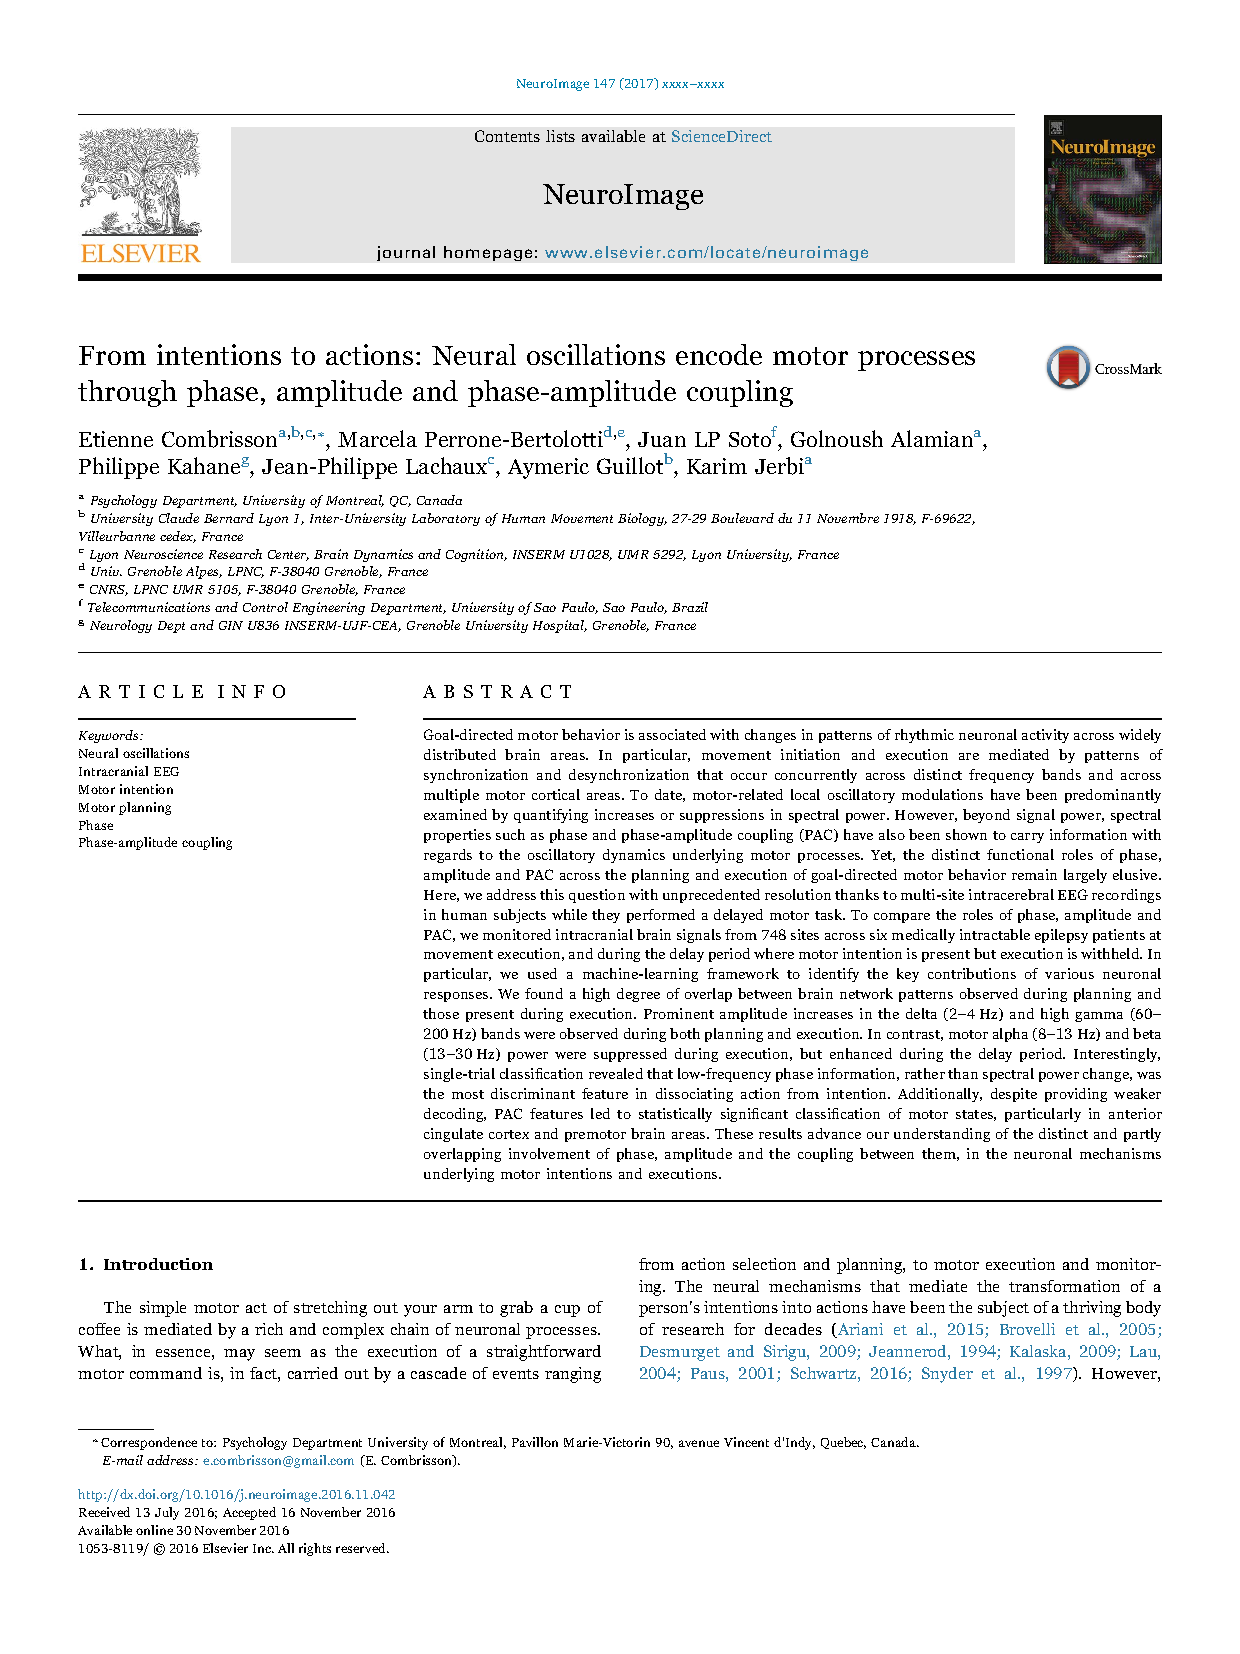
\includepdf[pages={1-29}]{Chap2/Etude2_Combrisson-etal-Encoding-Intention-Execution.pdf}


%!TEX root = ../main.tex
\part{�tude 3: D�codage des directions de mouvement pendant et avant l'ex�cution de mouvement de membres sup�rieurs}
\label{Etude3_decodage}


\chapter*{Introduction}
Mon introduction


%%% --------------------------
%%% Article
%%% --------------------------
\includepdf[pages={1-28}]{Chap3/Combrisson-etal_Decoding-Intention-Execution.pdf}


%!TEX root = ../main.tex
\part{�tude 4 : Tensorpac, logiciel Python de calcul de Phase-Amplitude Coupling}
\label{Etude4_tensorpac}
\pagestyle{headings}


\chapter*{Introduction}
Le \pacFR (PAC) est un marqueur qui mesure le degr�s de couplage entre la phase d'ondes lentes et l'amplitude d'ondes rapides. L'�valuation d'un couplage se fait de mani�re suivante :
\begin{itemize}    
    \item Extraction de la phase et de l'amplitude en utilisant soit des outils de filtrage suivi de la transform�e d'Hilbert, soit une transformation continue en ondelettes.
    \item Calcul du couplage entre ces deux signaux en utilisant une des m�thodologies existantes \citep{tort_measuring_2010,ozkurt_statistically_2012,canolty_high_2006}...
    \item Le PAC �tant une mesure sensible aux bruits, on construit une distribution de mesure de PAC pouvant arriver par chance.
    \item La v�ritable mesure de PAC est ensuite normalis�e par cette distribution de chance afin de minimiser le bruit.
\end{itemize}
Un nombre cons�quent de m�thodes ont �t� propos�es pour chacune de ces �tapes ce qui complique la comparaison et la reproductibilit�. De plus, toutes les publications introduisant de nouvelles m�thodes les pr�sentent en utilisant des vecteurs et ne fournissent pas l'adaptation matricielle ce qui ne prend pas en compte le format des donn�es (nombre de sujets, d'�lectrodes, d'essais...) et donc n'est pas du tout optimal d'un point de vue temps de calcul.\\
Dans ce contexte, nous avons mis en place une toolbox Python, \textit{Tensorpac}, d�di�e exclusivement au calcul du \pacFR. Dans cette toolbox les m�thodes sont impl�ment�es de fa�on modulaire ce qui signifie que l'utilisateur peut combiner les m�thodes existantes pour chacune des �tapes du calcul du PAC. D'autre part, \textit{Tensorpac} utilise des tenseurs permettant de g�n�raliser le calcul � partir de s�ries temporelles vers des donn�es multi-dimensionnelles. Cette impl�mentation en tenseurs est combin�e � du calcul en parall�le ce qui diminue encore le temps d'ex�cution et facilite l'envoie sur des serveurs de calcul. Ce paquet inclue �galement le calcul de comodulograme (soit en cherchant les couples (phase, amplitude) soit en fixant l'un des deux et en faisant varier la largeur de bande de l'autre), statistiques et la visualisation. Pour finir, \textit{Tensorpac} est distribu� sous une licence BSD et peut �tre t�l�charger sur Github \footnotemark[1] et nous fournissons �galement une documentation d�taill�e \footnotemark[2].

\footnotetext[1]{\url{https://github.com/EtienneCmb/tensorpac}}
\footnotetext[2]{\url{https://etiennecmb.github.io/tensorpac/}}


%%% --------------------------
%%% Article
%%% --------------------------
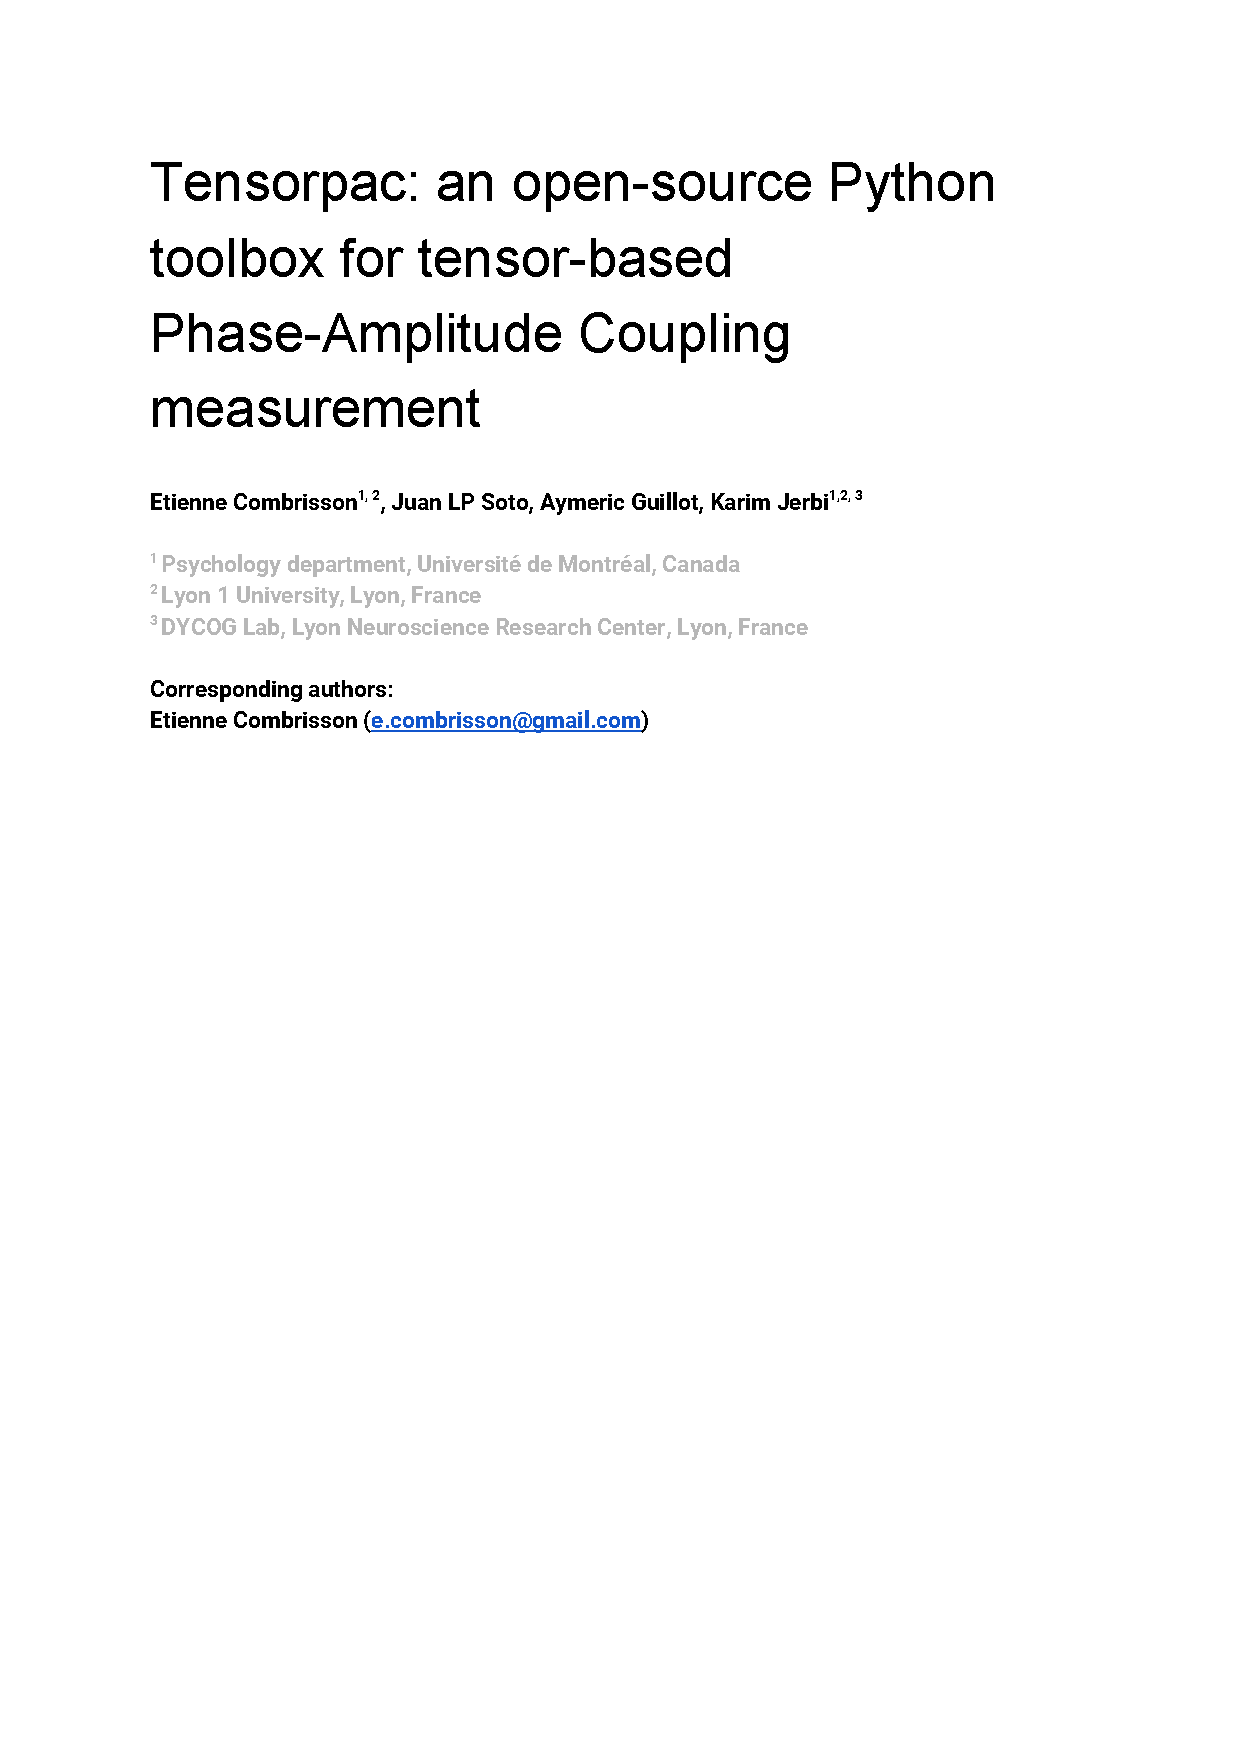
\includepdf[pages={1-18}]{Chap4/combrisson_2017_tensorpac.pdf}
\part{�tude 5: d�codage des �motions}
\label{Etude5_emotions}


\chapter*{Introduction}
blabla Intro

\vspace{1\baselineskip}
Blabla �tude


%%% --------------------------
%%% Article
%%% --------------------------
%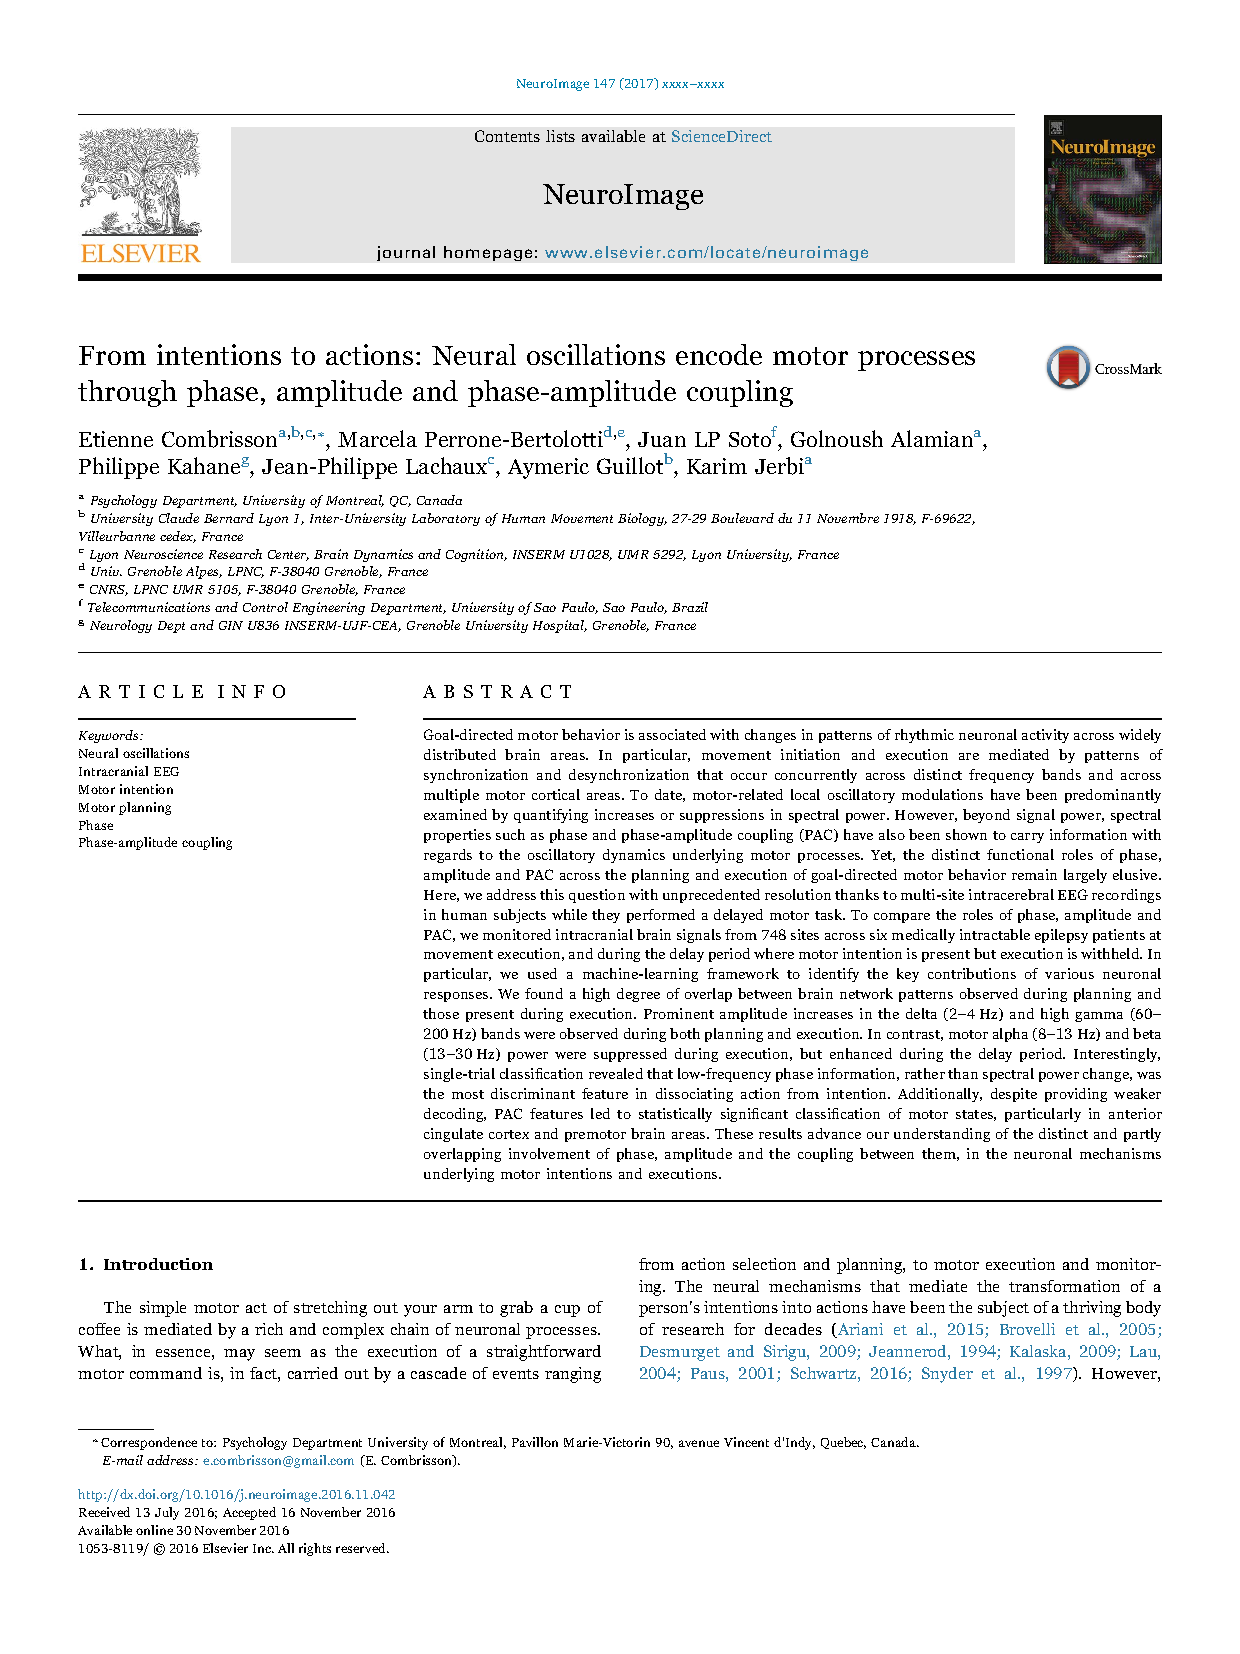
\includepdf[pages={1-29}]{Chap2/Etude2_Combrisson-etal-Encoding-Intention-Execution.pdf}




% ==================================================================
% CONCLUSION
\makeatletter
\renewcommand*{\toclevel@chapter}{-1}
\part{Discussion, conclusion et perspectives}
% \addcontentsline{toc}{chapter}{Conclusion g�n�rale}
\pagestyle{headings}

\chapter*{Discussion}

% Paragraphe 1-Vue d'ensemble de ce travail de th�se: Il s'est d�clin� en deux composante: Une contribution empirique [articles 2 et 3] et des contributions m�thodologiques (� la fois th�oriques [article 1] mais aussi en temre de d�veloppement logiciel [articles 4-6].

Ce travail de th�se s'articule autour de deux grands axes, (\textit{1}) un apport empirique permettant d'am�liorer notre compr�hension du r�le des composantes d'amplitude, de phase et de couplage phase-amplitude lors d'une t�che motrice dirig�e (articles 2 et 3). Nous avons utilis� des algorithmes de classification pour identifier les marqueurs les plus pertinents, (\textit{2}) un apport m�thodologique que ce soit d'un point de vue th�orique pour mieux comprendre la notion de seuil de chance en \textit{machine-learning} (article 1) et pratique via l'impl�mentation de plusieurs logiciels d'analyse et de visualisation (articles 4-6). \\

% Paragraphe 2-R�sum� des r�sultats les plus saillants obtenus dans les �tudes empiriques (articles 2 et 3)

Les deux articles empiriques partagent une m�me m�thodologie : l'utilisation des algorithmes de \textit{machine-learning} pour identifier les marqueurs de puissance, de phase et de PAC susceptibles de d�coder les �tats moteurs (article 2 cf. \ref{Etude2_encodage}) ou les directions motrices (article 3 cf. \ref{Etude3_decodage}). Cette premi�re �tude a permis de mettre en �vidence une augmentation significative de couplage $\alpha/\gamma$ durant la phase de repos qui s'att�nue ensuite durant l'ex�cution. D'un point de vue d�codage, la composante de phase tr�s basse fr�quence (\textit{VLFC}, $<1.5hz$) est le marqueur ayant montr� les plus forts taux de d�codage � travers toutes les conditions classifi�es (\textit{Repos Vs Pr�p.}, \textit{Repos Vs Exec.}, \textit{Pr�p. Vs Exec.}, \textit{Repos Vs Pr�p. Vs Exec.}). Dans une moindre mesure, le PAC pr�sente lui aussi des d�codages significatifs pour diff�rencier ces �tats moteurs ce qui n'est pas le cas pour diff�rencier les directions (article 3 cf \ref{Etude3_decodage}). En effet, le d�codage \textit{Up Vs Down Vs Left Vs Right} est majoritairement possible via des marqueurs de puissance. Durant l'ex�cution, la puissance des oscillations $\gamma$ permet de clairement diff�rencier les modulations � travers les directions dans les r�gions motrices et pr�-motrices. Plus important encore, le m�me ph�nom�ne a lieu lorsque la puissance dans la bande $\alpha$ dans le cortex pr�-moteur et frontal est utilis�e. Pris ind�pendamment, ces deux marqueurs en utilisation unique permettent d'obtenir des d�codages significatifs ($~70\%$ pour l'ex�cution et $~50\%$ durant la pr�paration). Pour finir, nous avons combin� plusieurs algorithmes de \textit{feature selection} ce qui a permis d'atteindre des d�codages proches de $90\%$ pour diff�rencier les quatre directions � la fois durant l'ex�cution et la pr�paration motrice. \\

% Paragraphe 3-Mettre en valeur la nouveaut�/originalit� de ces r�sultats (� quel point c'est diff�rent de ce qu'avait fait les autres chercheurs jusqu'ici?)

PARAGRAPHE DE CE QUI EST VRAIMENT NOUVEAU. \\

% Paragrpahe 4-Regard critique sur les 2 �tudes en intra: Les limitations de ces donn�es (nombre de patients, le fait qu'il s'agit de patient, le fait que les electrodes se trouvent � des endroits diff�rents � travers les patients, le fait que le d�lain'�tait pas variable, le fait qu'on avait pas acc�s syst�matique � l'onset du mouvement, etc etc).

Ces deux �tudes ont un certain nombre de limitations. Tout d'abord, les donn�es intracr�niennes �tant relativement rares, nous n'avons acc�s qu'aux donn�es de six sujets, chacun ayant approximativement une centaine d'�lectrodes. Au total, ces 6OO points d'enregistrement offrent une couverture partielle des r�gions c�r�brales. De plus, ces sujets souffrent d'une forme d'�pilepsie pharmacor�sistante ce qui limite la possibilit� de g�n�raliser � des sujets sains. L'implantation des sites intracr�niens �tant li�e � la localisation du foyer �pileptog�ne, il en r�sulte une implantation propre � chaque sujet et donc, d'une part il est tr�s difficile de pouvoir g�n�raliser le comportement d'un site en particulier puisqu'il est possible qu'il soit le seul dans cette r�gion et d'autre part, l'implantation n'�tant pas sym�trique elle ne permet pas d'�tudier l'effet controlat�ral et ipsilat�ral. La t�che utilis� pour mener � bien ces deux �tudes a �galement des limitations. Tout d'abord, tout les \textit{timing} sont fixes et donc, en l'absence de d�lais variables, il est tout � fait envisageable que les sujets puissent anticiper le d�but d'une phase au fur et � mesure que la t�che avance. De plus, le design de la t�che ne permet pas de conclure clairement sur le type de processus d�cod�s. En effet, on est en droit de se demander si l'on d�code une v�ritable pr�paration/ex�cution de mouvements ou un processus attentionnel, visuomoteur, s�lection spatiale ou d'imagerie motrice. Pour finir, apr�s l�apparition d'un signal visuel, les donn�es ne permettaient pas d'avoir acc�s au d�but du mouvement. Ainsi, l'activit� neuronale contenue dans les tanches temporelles qui suivent directement l'apparition du signal visuel peut contenir des �v�nements diff�rents d� � la variabilit� du temps de r�action d'un essais � l'autre. Les outils de \textit{machine-learning} �tant justement entra�n�s � travers les essais, l'alignement sur le \textit{go-signal} pourrait alors d�grader la performance de classification. \\

% Paragraphe 5-Pour quoi est-ce que malgr�s ces limitations nous avons confiance dans les r�sultats obtenus?

Pour pouvoir g�n�raliser les �tudes 2 et 3 aux sujets sains, les �lectrodes proches des yeux ou contenant une activit� �pileptiforme sont syst�matiquement rejet�es. De plus, les analyses sont appliqu�es � travers les essais ce qui permet de minimiser l'activit� c�r�brale qui n'est pas directement reli�e � la t�che. M�me si les six sujets offrent une couverture partielle, ils ont �t� s�lectionn�s pour leur implantation pr�-frontale, frontale et pari�tale \cad l� o� l'on attend les meilleurs r�sultats de d�codage d'une t�che motrice. L'�tude de la lat�ralit� est une limitation propre � tout les enregistrements invasifs et devrait donc �tre trait� avec des enregistrements d'EEG de scalp ou de MEG. L'impact du d�lai fixe et de l'alignement sur le \textit{go-signal} de la t�che ont �t� minimis�s de fa�on diff�rentes dans chacune de ces deux �tudes. Dans la premi�re (cf. \ref{Etude2_encodage}) la fen�tre de d�codage consid�r�e pour diff�rencier les �tats moteurs se situent 500ms apr�s le \textit{go-signal} et donc, devrait limiter l'utilisation d'une activit� neuronale non-pertinente. Dans le second article (cf. \ref{Etude3_decodage}, le d�codage des directions se fait dans un esprit \textit{temps-r�el}. Un classifieur est syst�matiquement r�-entra�n� puis test� dans les diff�rentes fen�tres temporelles d�finies (67 au total), du d�but du repos � la fin de l'ex�cution. En cons�quence, seule 2/67 fen�tres qui suivent les deux indications visuelles peuvent potentiellement montrer des d�codages plus bas. \\

% Paragraphe 6-R�sumer l'apport de d�veloppement logiciel (re-mentionner les packages, et le nombre de lignes de code par package). Indiquer qu'ils peuvent �tre utilis�s pour des applications diverses et vari�es au-del� de ce pourquoi ces outils ont �t� d�velopp�s au d�part (les donn�es motrices en intra etc.). Indiquer en quelques lignes des d�veloppments futurs pr�vus pour certains de ces outils et le d�sir d'encourager d'autres personnes � contribuer activement au d�veloppment de ces outils das un esprit de partage/communautaire etc  (ce ne sont que des id�es bien sur)

Pour finir, tout les r�sultats d'analyses et de visualisation de cette th�se sont issus des logiciels Python open-source d�velopp�s � cet effet. \textit{Brainpipe} ($7899$ lignes) permet d'extraire des marqueurs de l'activit� neuronale (tel que l'amplitude, puissance, phase \dots) et de les classifier en utilisant \textit{Scikit-Learn}. \textit{Tensorpac} ($2230$ lignes), autre paquet Python open-source, permet de calculer le \pacFR avec une impl�mentation modulaire des m�thodes le tout reposant sur des calculs bas�s sur des tenseurs et mise en parall�le. Pour finir \textit{Visbrain} ($30771$ lignes) permet d'obtenir de visualiser de nombreux types de donn�es (pour du \textit{data-mining}, avec cerveau MNI semi-transparent, donn�es de sommeil \dots). Ces trois principaux paquets ont d'abord �t� d�velopp�s pour couvrir nos besoins. Puis, dans un d�sir de partager nos outils, ils ont �t� enti�rement reformat�s pour �tre utilisable par d'autre. \textit{Brainpipe} �tant le premier paquet d�velopp�, pourrait �tre tr�s largement am�lior� (surtout dans la gestion des dimensions des donn�es et de la m�moire RAM). \textit{Tensorpac} et \textit{Visbrain} n'ont pas ce soucis puisqu'ils ont �t� entam�s apr�s une connaissance plus mature du langage Python. Toutefois, de nombreuses autres m�thodologies pourraient �tre ajout�es � \textit{Tensorpac}, certaines �tant plus dur que d'autres � �tre impl�ment�es en tenseurs. Pour finir, \textit{Visbrain} � une longue feuille de route de pr�vue pour son d�veloppement futur, incluant de nombreuses refontes, am�liorations et surtout l'ajout de nouveaux modules de visualisations. Quoi qu'il en soit, avec leur qualit�s et leurs d�fauts, ces trois logiciels viennent avec un code extr�mement comment�, des datasets et exemples et des documentations. Mon plus grand souhait �tant que d'autres personnes participent � faire avancer ces projets tout en conservant l'id�e principale, un partage libre pour une science ouverte. 

\chapter*{Conclusion et perspectives futurs}

[1/2 page suffira]

2 id�es � d�velopper

(i) Un truc du genre "Taken together, this body of research advances our understanding of the role of oscillatory power, phase and PAC in goal-directed behavior, and provides efficient open-source packages for the scientific community to replicate and extend this research."

(ii) Proposer des pistes prometteuses pour l'avenir: Par exemple le fait de s'orienter d�finitivement vers des �tudes du syst�me moteur dans de grandes cohortes de sujets (via le data sharing et �tude multi-centriques) et via le open-science et le partage des outils d'analyses pou rrenforcer la reproductiblit� des r�sultats etc.


% ==================================================================
% ANNEXES
\let\cleardoublepage\clearpage
\appendix
\renewcommand*{\toclevel@section}{0}
\pagestyle{plain}

% *****************************************************************
%                   BCI MAP
% *****************************************************************
\section{Cartes des Interfaces Cerveau-Machine \citep{graimann_braincomputer_2009}}
\begin{figure}[H]
	\centering
	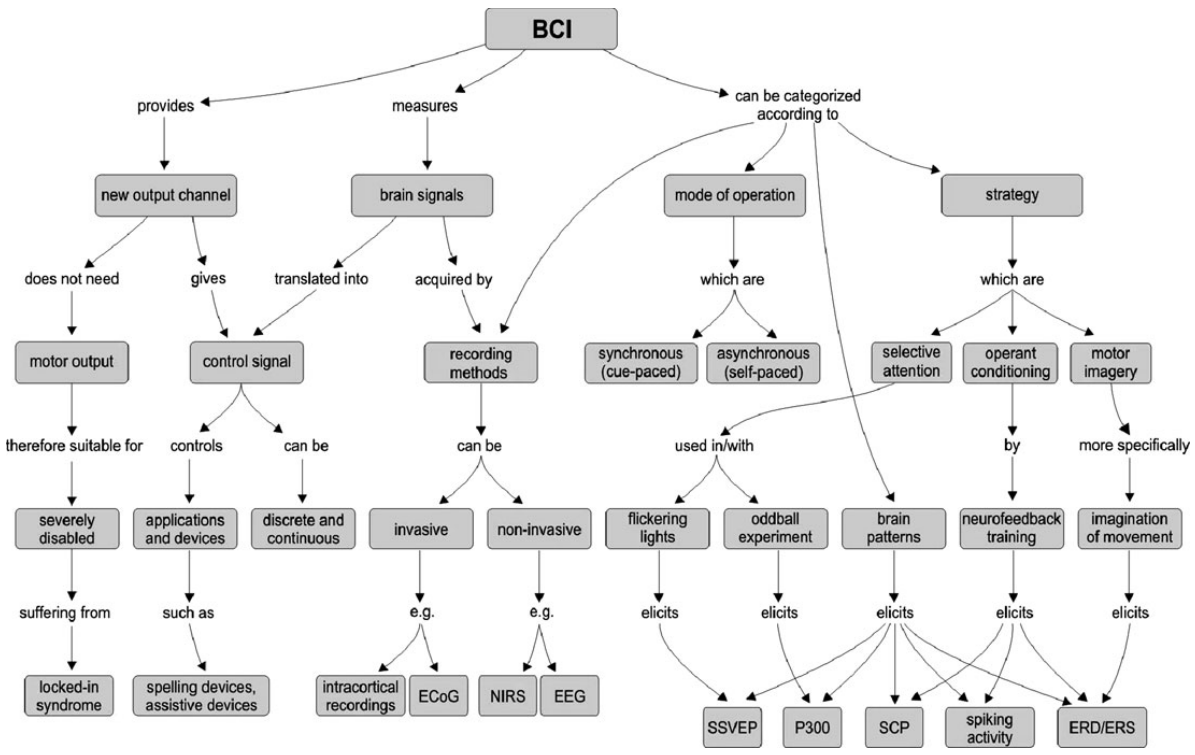
\includegraphics[scale=0.5,angle=-90]{./figures/Grainmann_2002_ICM_map}
	\caption{Cartes des Interfaces Cerveau-Machine \citep{graimann_braincomputer_2009}}
	\label{bci_map}
\end{figure}

% *****************************************************************
%                   BCI COMPETITION
% *****************************************************************
\section{Jeux de donn\'{e}es en libre acc\`{e}s (\textit{BCI competition})}
\begin{figure}[H]
	\begin{tabular}{|c|c|c|p{8cm}|}
		% COMPETITION II
		\hline
		\multicolumn{4}{|c|}{\href{http://www.bbci.de/competition/ii/}{BCI Competition II}} \tabularnewline
		\hline
		Set & N-Classes & Channel & Challenge \tabularnewline
		\hline
		Ia/Ib & 2 & 6-EEG & Decide whether the subject tried to produce cortical negativity or cortical positivity \tabularnewline
		\hline
		IIa & 4 & 64-EEG & Provide the intended target of the feedback test trials  \tabularnewline
		\hline
		IIb & 36 & 64-EEG & Estimate to which letter of a 6-by-6 matrix with successively intensified rows resp. columns the subject was paying attention to  \tabularnewline
		\hline
		III & 2 & 3-EEG & Provide a continuous output that could be used for a BCI- feedback \tabularnewline
		\hline
		IV & 2 & 28-EEG & Predict the laterality of upcoming finger movements (left vs. right hand) 130 ms before keypress \tabularnewline
		\hline

		% COMPETITION III
		\multicolumn{4}{|c|}{\href{http://www.bbci.de/competition/iii/}{BCI Competition III}} \tabularnewline
		\hline
		I & 2 & 64-ECoG & Cued motor imagery (left pinky, tongue) from one subject \tabularnewline
		\hline
		II & 36 & 64-EEG & Estimate to which letter of a 6-by-6 matrix with successively intensified rows resp. columns the subject was paying attention to \tabularnewline
		\hline
		IIIa & 4 & 60-EEG & Cued motor imagery with 4 classes (left hand, right hand, foot, tongue) from 3 subjects. Measure: kappa-coefficient \tabularnewline
		\hline
		IIIb & 2 & 2-EEG & Cued motor imagery with online feedback with 2 classes (left hand, right hand). Measure: mutual information \tabularnewline
		\hline
		IVa/IVb/IVc & 2 & 118-EEG & Cued motor imagery with 2 classes (right hand, foot) from 5 subjects \tabularnewline
		\hline
		V & 3 & 32-EEG & Cued mental imagery with 3 classes (left hand, right hand, word association) from 3 subjects \tabularnewline
		\hline
	
		% COMPETITION IV
		\multicolumn{4}{|c|}{\href{http://www.bbci.de/competition/iv/}{BCI Competition IV}} \tabularnewline
		\hline
		I & 2 & 64-EEG & Motor imagery (2 classes of left hand, right hand, foot) \tabularnewline
		\hline
		IIa & 4 & 22-EEG & Cued motor imagery (left hand, right hand, feet, tongue)   \tabularnewline
		\hline
		IIb & 2 & 3-EEG & Cued motor imagery (left hand, right hand)   \tabularnewline
		\hline
		III & 4 & 10-MEG & Decoding directions of finger/hand/wrist movements \tabularnewline
		\hline
		IV & 5 & 64-ECoG & Discrimination of movements of individual fingers \tabularnewline
		\hline
	\end{tabular}
	\caption{Jeux de donn\'{e}es en libre acc\`{e}s (\textit{BCI competition})}
	\label{annexe_bci_competition}
\end{figure}

% *****************************************************************
%                   COMPARATIF PAC
% *****************************************************************
\section{Comparatif de m\'{e}thodes PAC \citep{tort_measuring_2010}}
\begin{figure}[H]
	\centering
	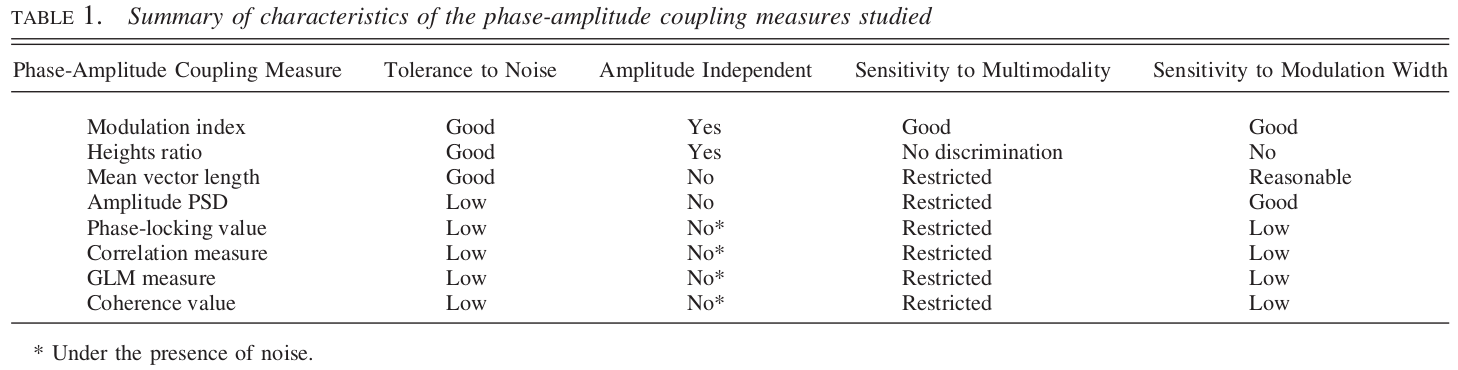
\includegraphics[scale=0.4,angle=-90]{./figures/PAC_methods_comparison}
	\caption{Comparatif de m\'{e}thodes PAC \citep{tort_measuring_2010}}
	\label{comp_pac}
\end{figure}

% *****************************************************************
%                   CLASSIFICATION PIPELINE
% *****************************************************************
\section{Pipeline standard de classification}
\begin{figure}[H]
	\centering
	\makebox[\textwidth][c]{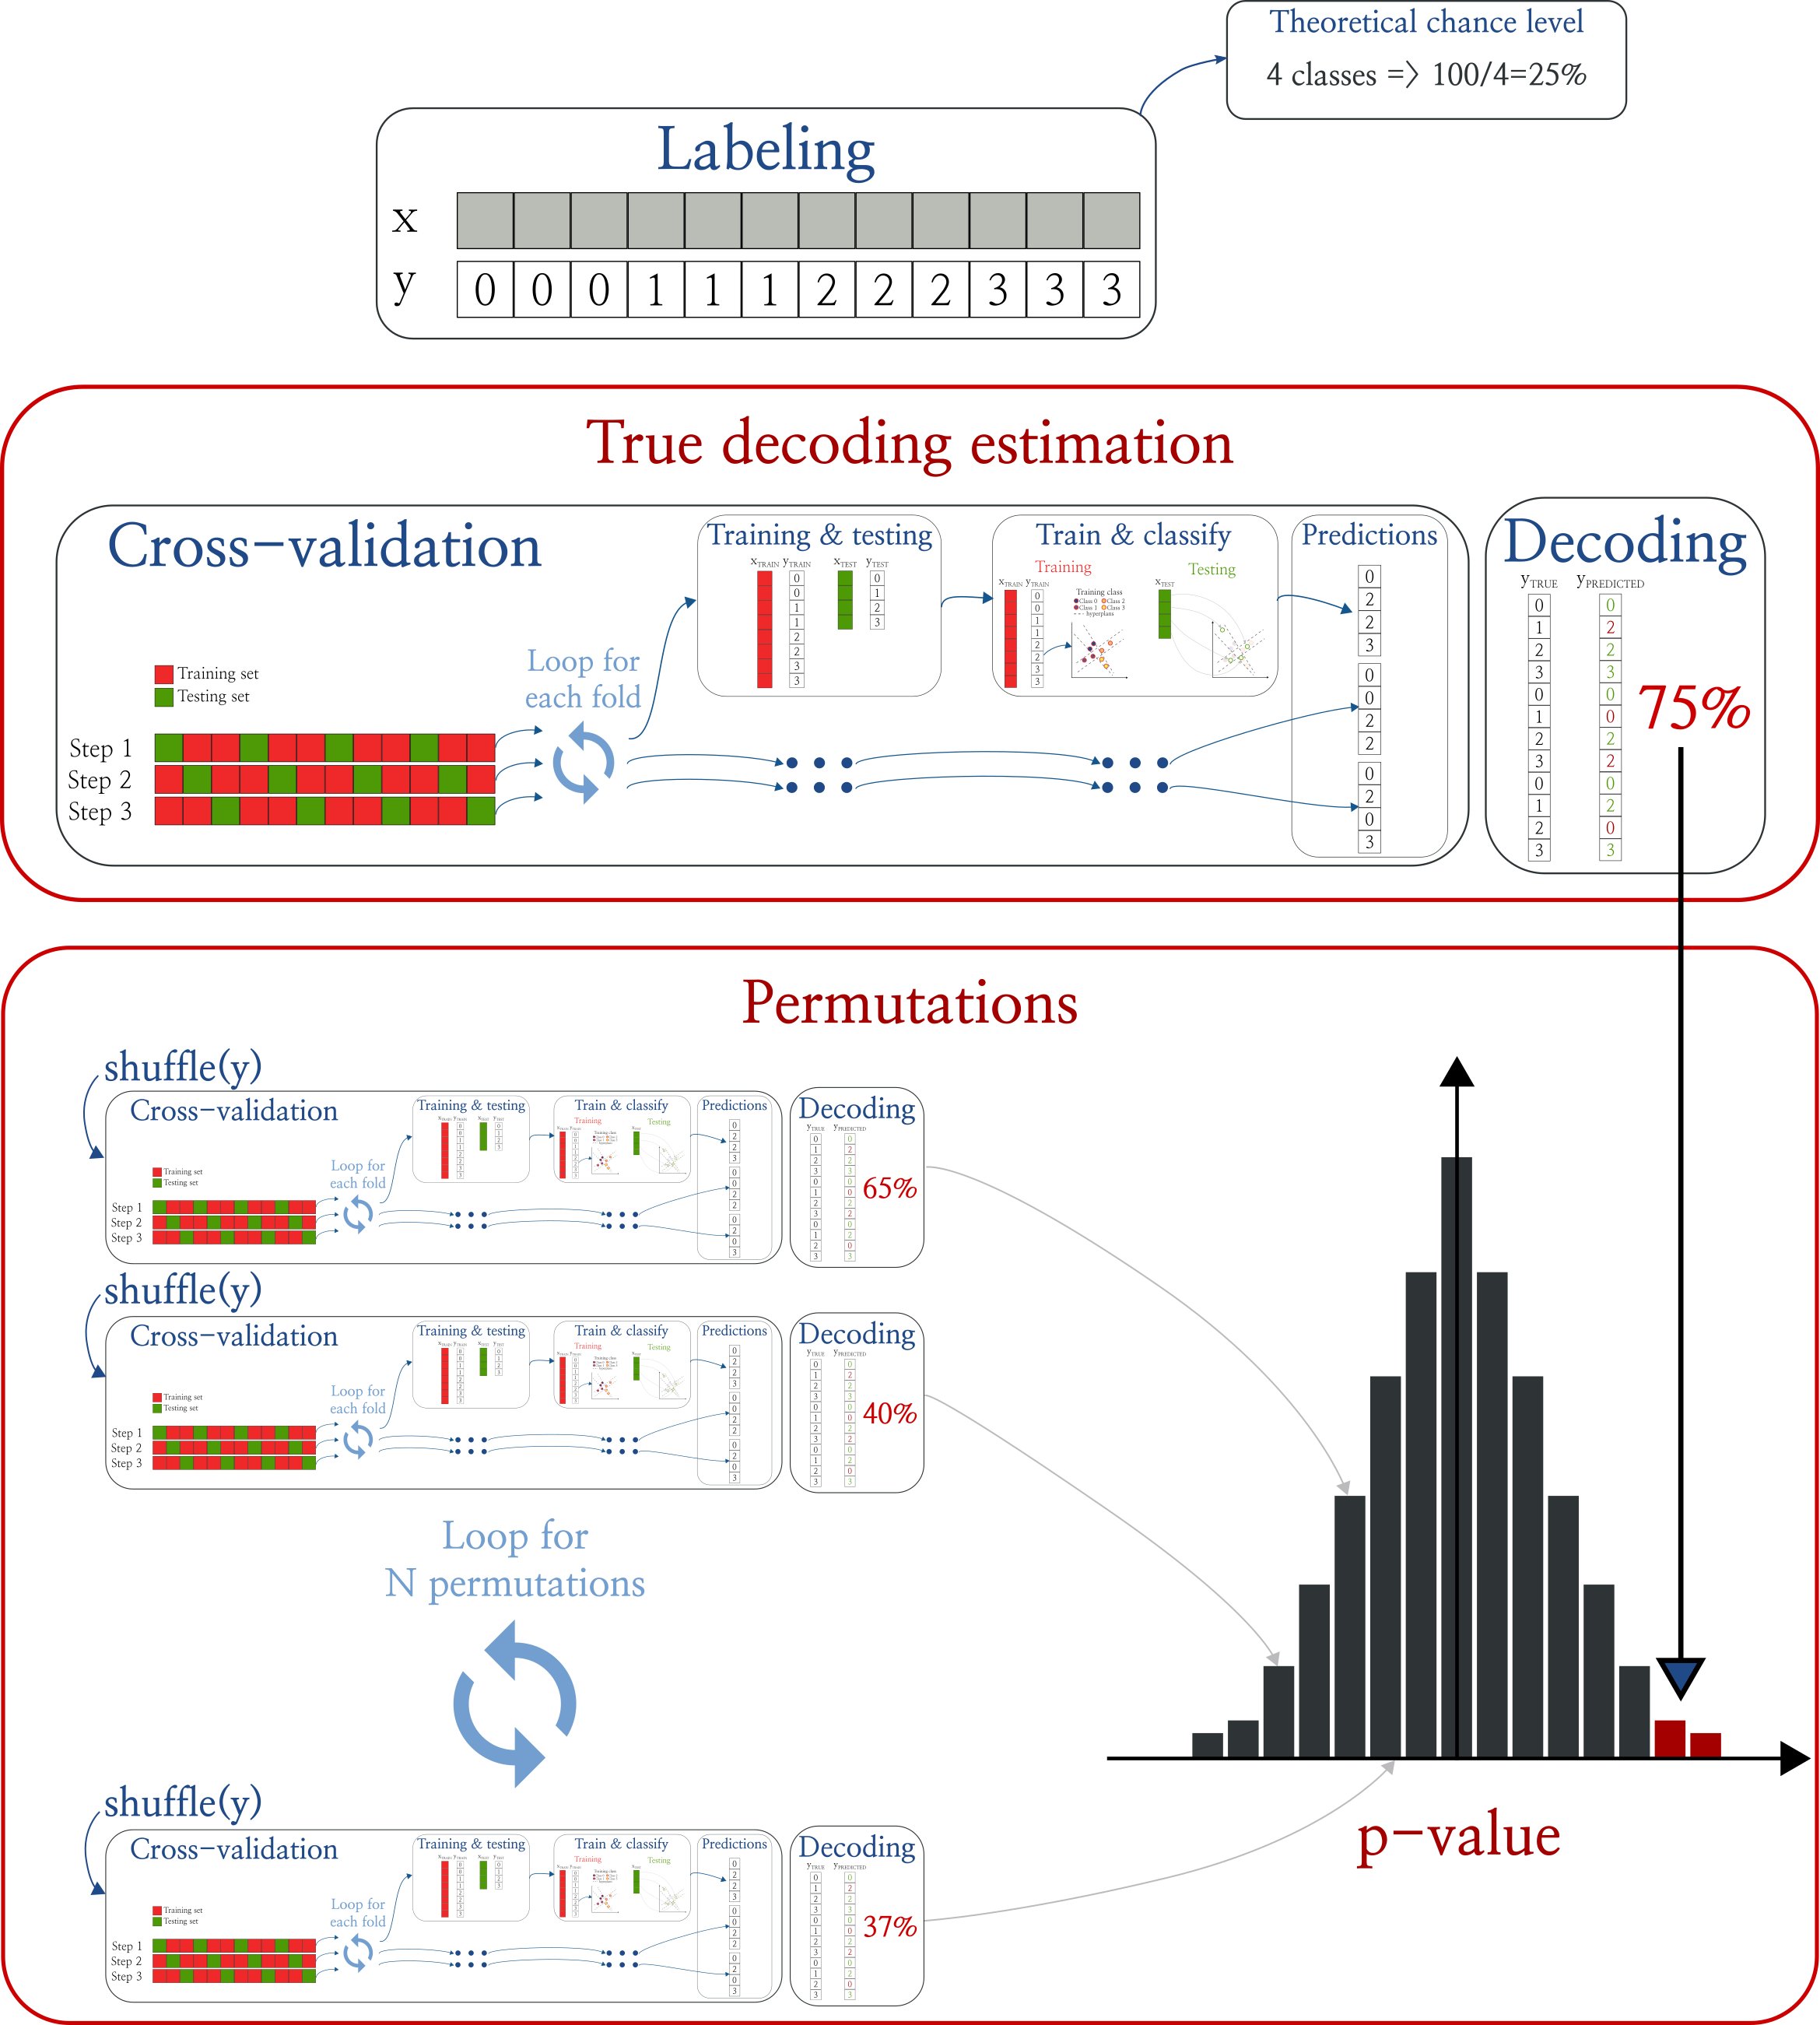
\includegraphics[scale=0.9]{./figures/clf_pipeline}}
	\caption{Pipeline standard de classification}
	\label{clf_pip}
\end{figure}

% *****************************************************************
%                   COMPARATIF CLASSIFIEURS
% *****************************************************************
\section{Comparatif de classifieurs \citep{scikit-learn}}
\begin{figure}[H]
	\centering
	\makebox[\textwidth][c]{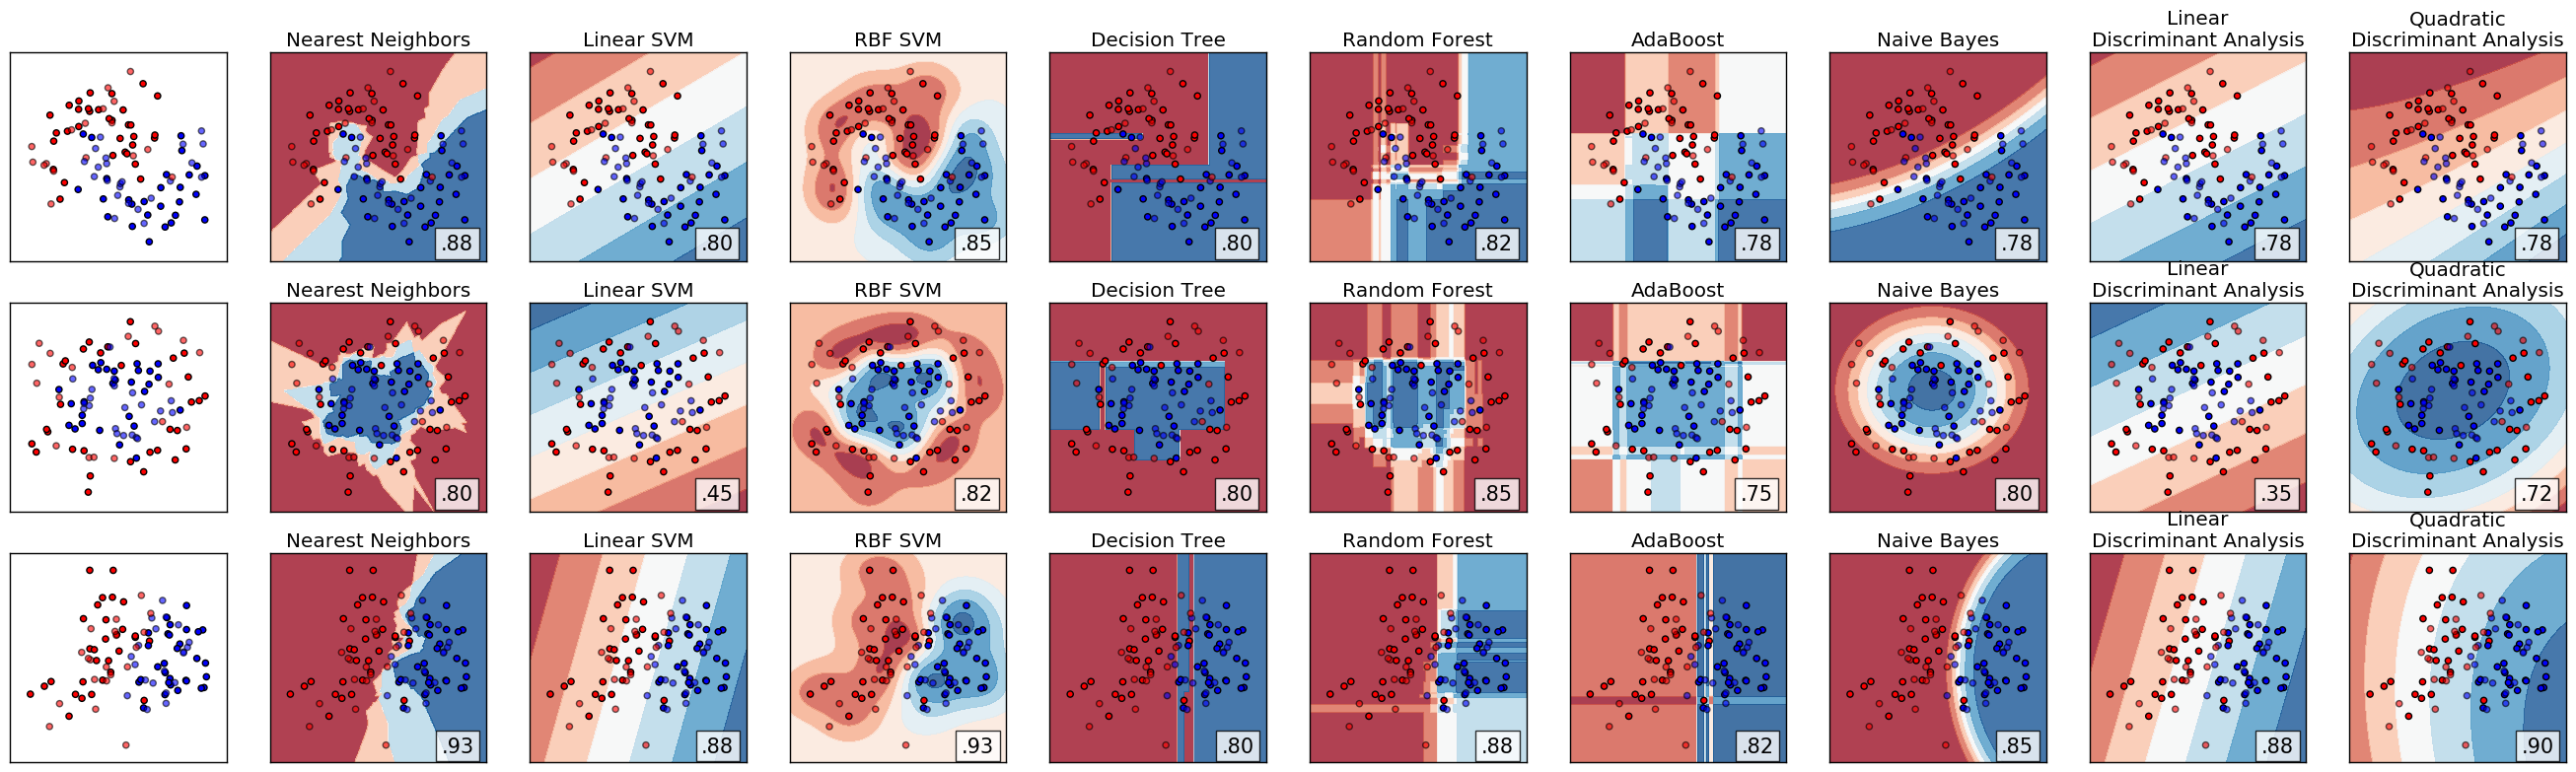
\includegraphics[scale=0.35,angle=-90]{./figures/classifier_comp}}
	\caption{Comparatif de classifieurs \citep{scikit-learn}}
	\label{comp_clf}
\end{figure}


% *****************************************************************
%                   SCHEMA IMPLANTATION
% *****************************************************************
\section{Exemple de sch\'{e}ma d'implantation}
\begin{figure}[H]
	\centering
	\makebox[\textwidth][c]{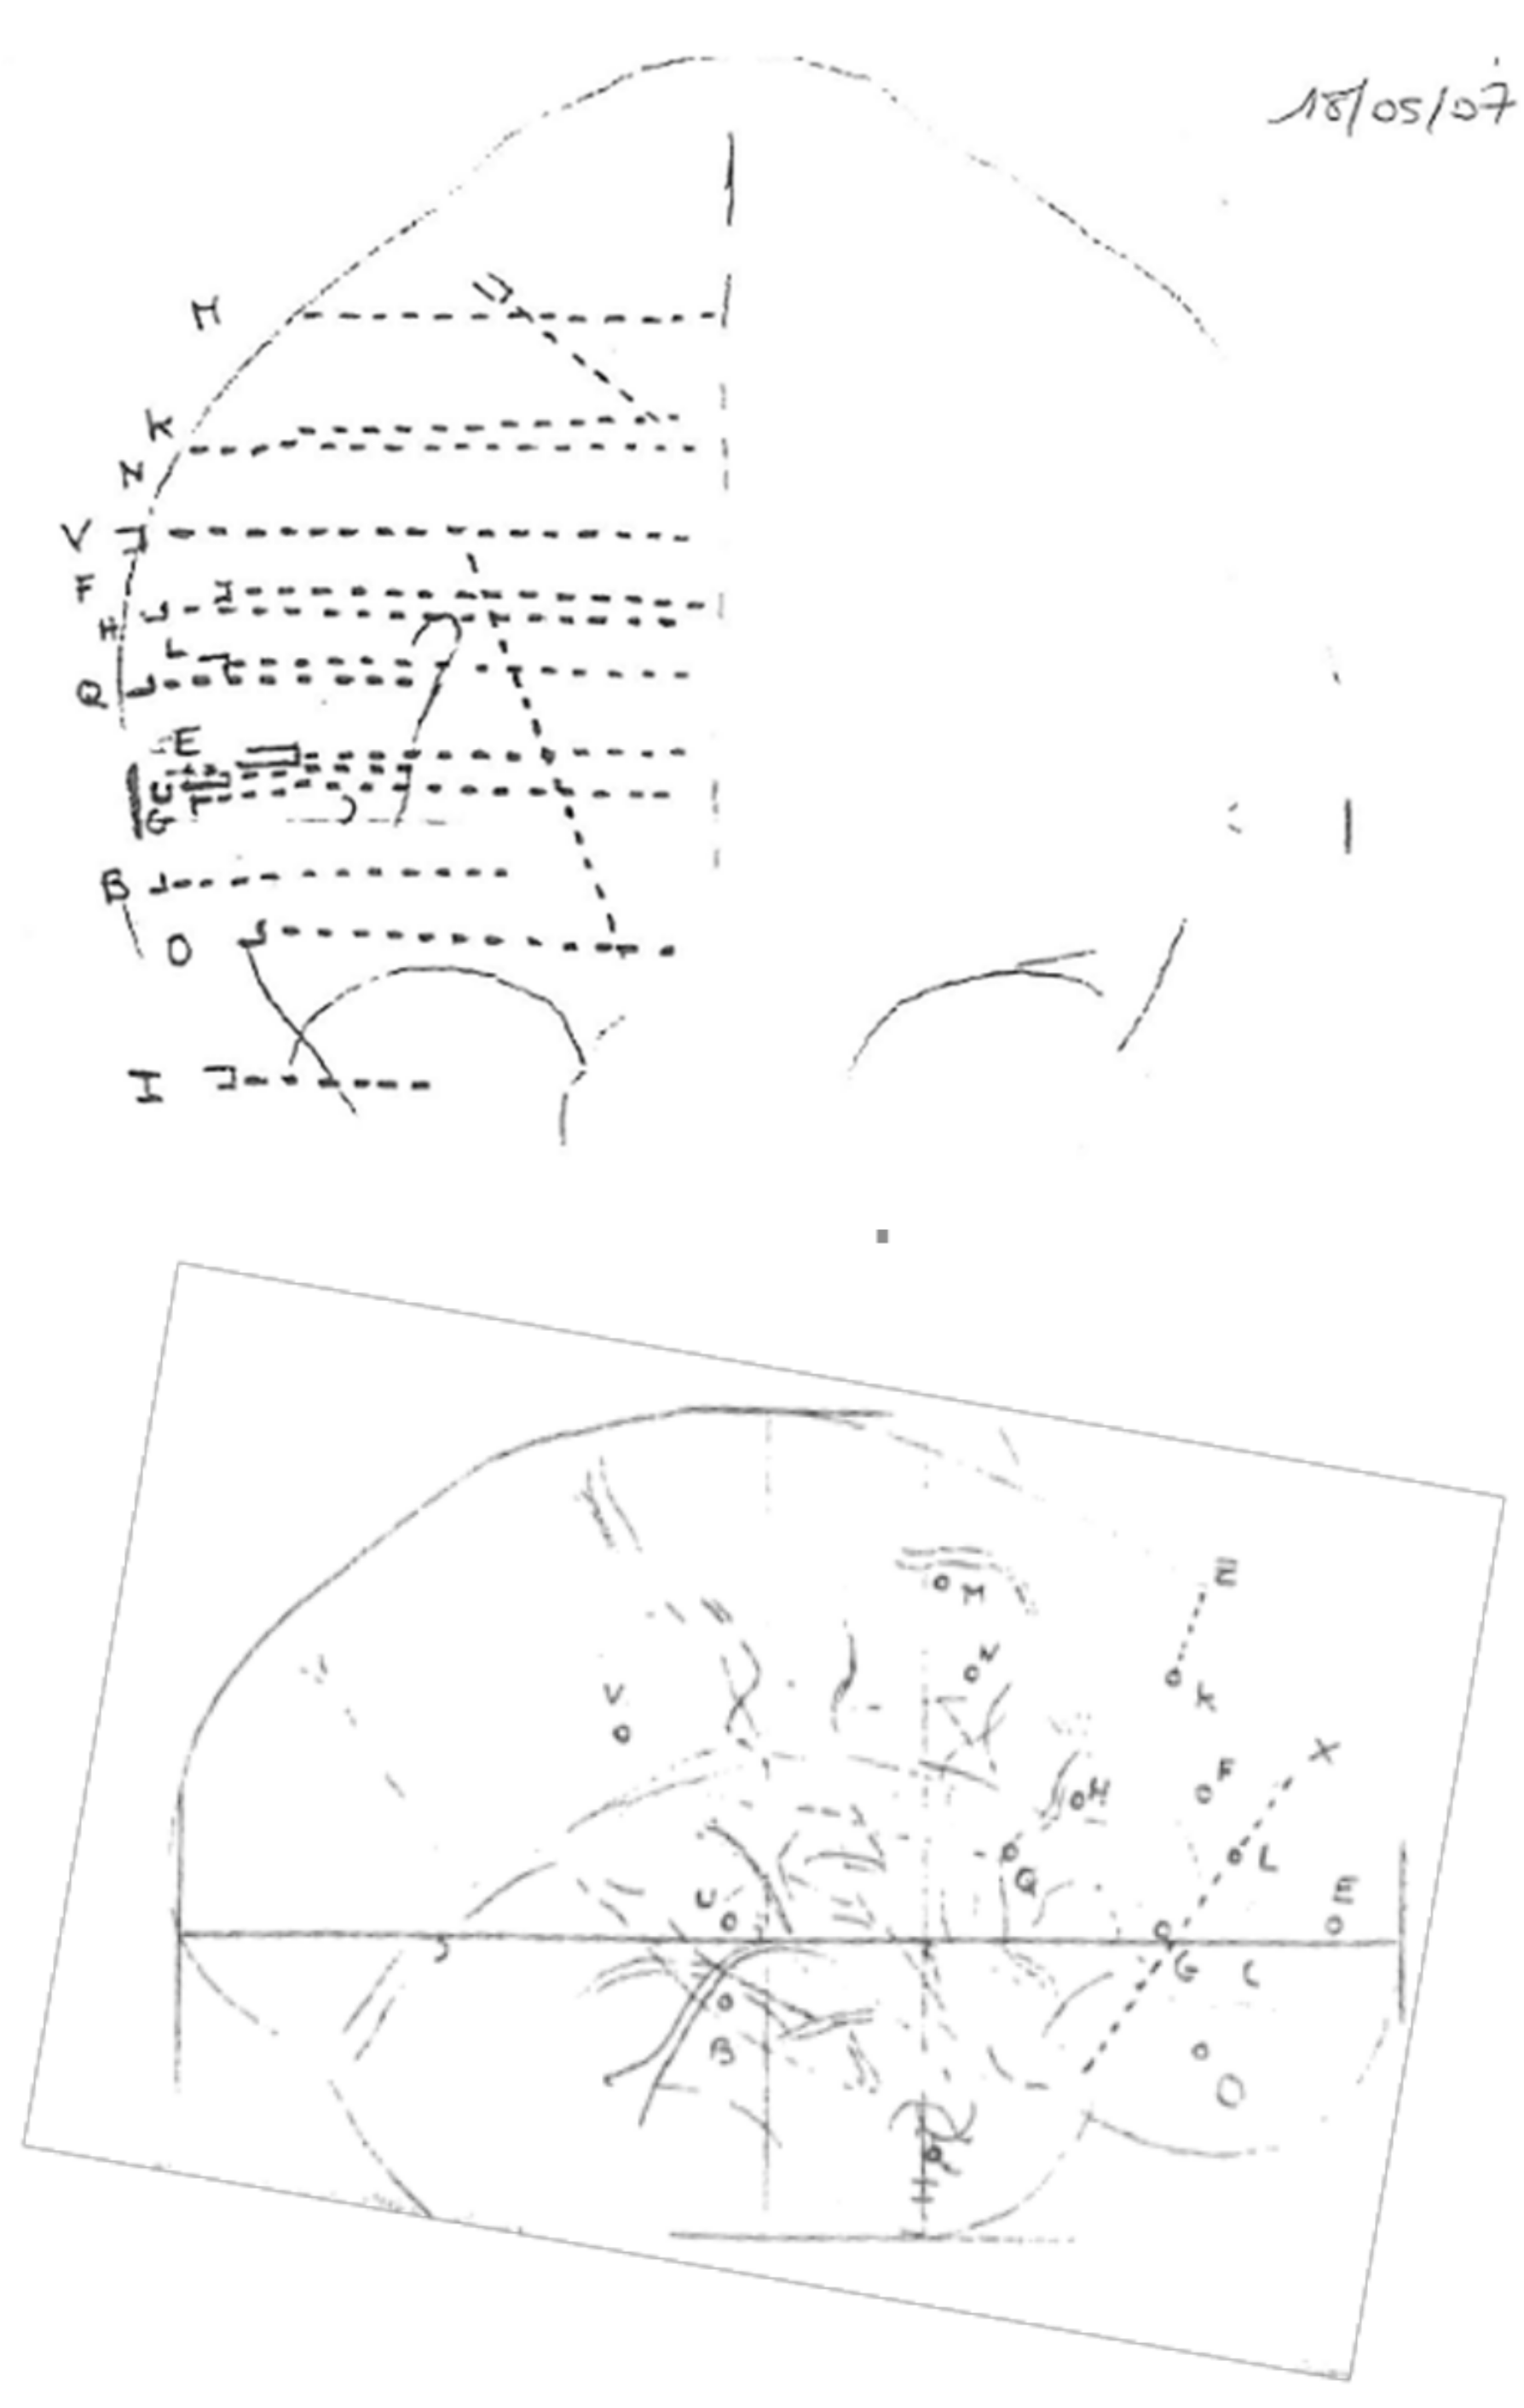
\includegraphics[scale=1]{./figures/schema-implantation_annexe}}
	\caption{Exemple de sch\'{e}ma d'implantation}
	\label{schema_implantation}
\end{figure}

% *****************************************************************
%                   DOCUMENTATION DE BRAINPIPE
% *****************************************************************
\section{Documentation de brainpipe}
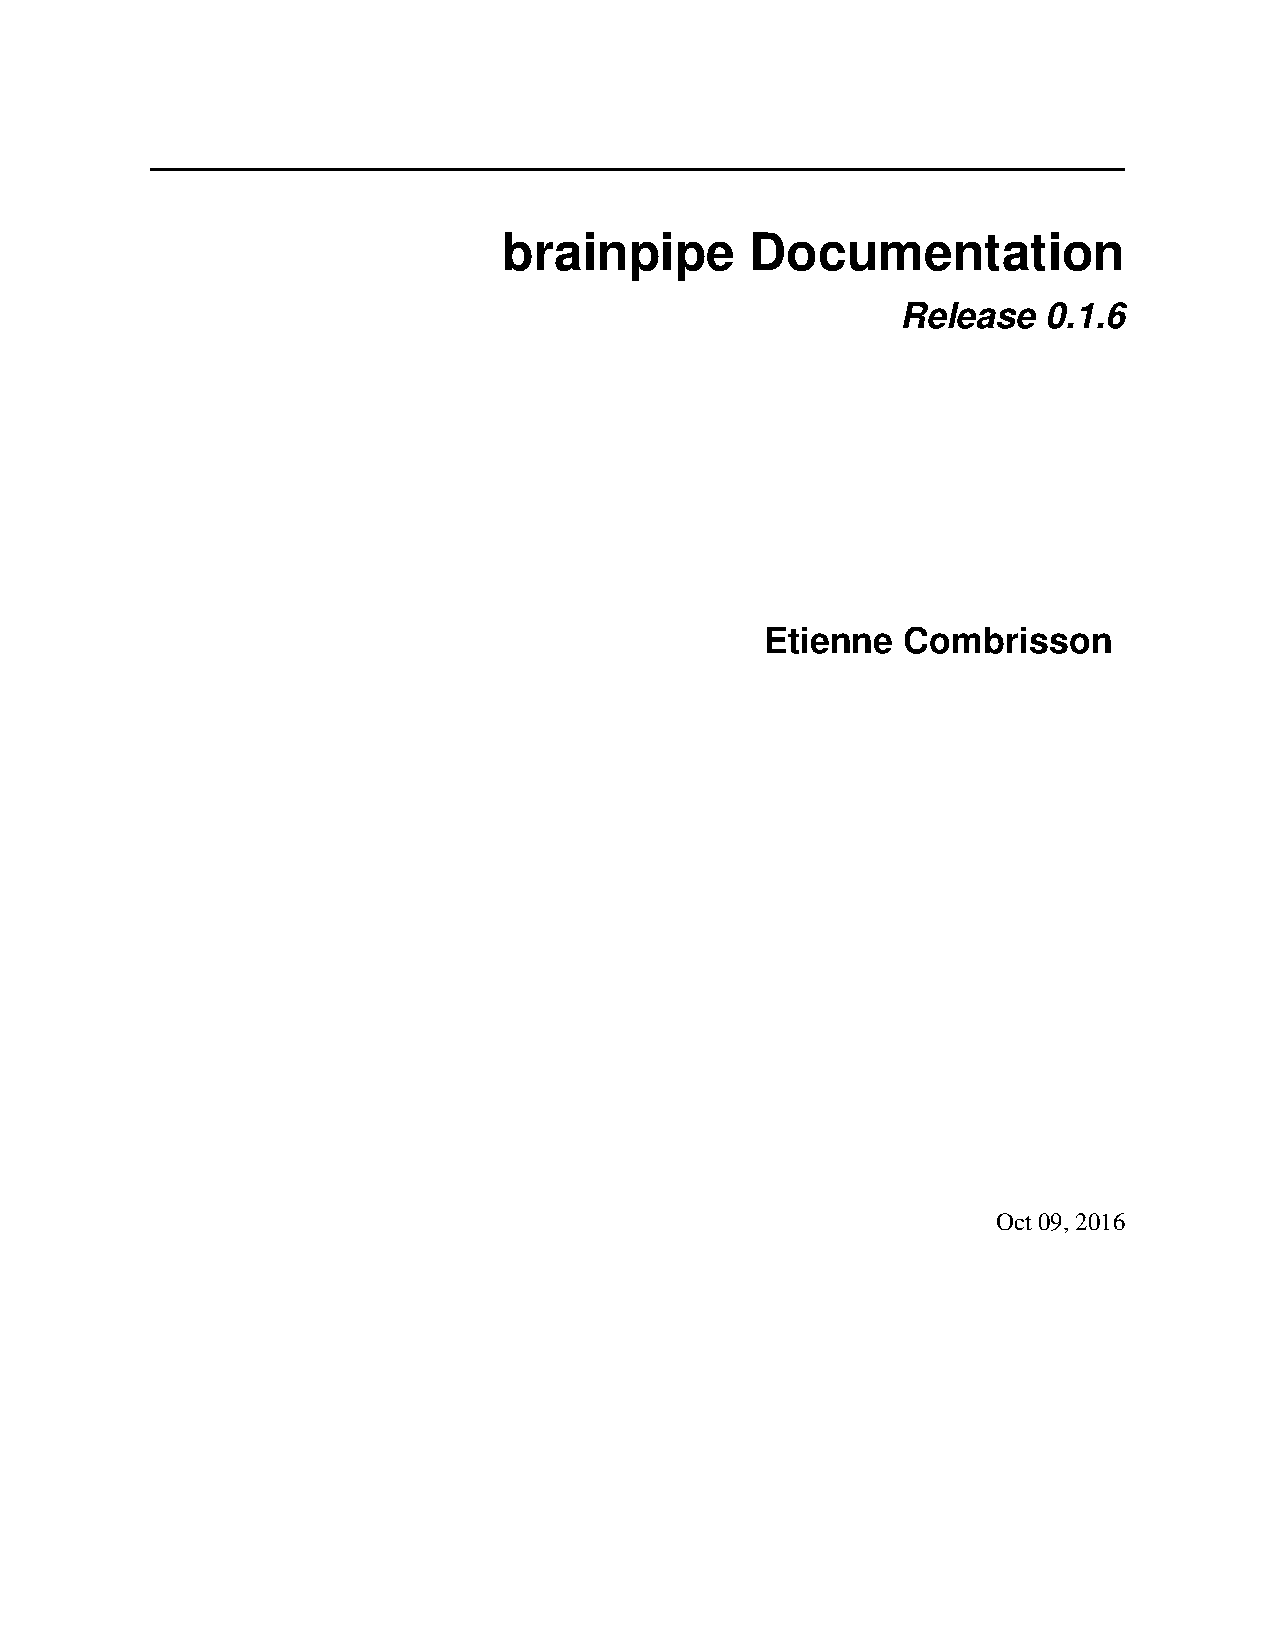
\includepdf[pages={1-69}]{Annexes/brainpipe.pdf}

 
% ==================================================================
% BIBLIOGRAPHIE
\makeatletter
\renewcommand*{\toclevel@chapter}{-1}
\backmatter
\bibliographystyle{apalike}
\bibliography{Manuscrit}
 
% ==================================================================
% COLOPHON
%\colophon{Ce document a �t� pr�par� � l'aide de l'�diteur de texte GNU
%  Emacs et du logiciel de composition typographique \LaTeXe.}
 
% ==================================================================
% COUVERTURE : RESUME ET MOTS-CL�S
\abstractpage


\end{document}
%%% Local Variables:
%%% mode: latex
%%% TeX-master: t
%%% End:
